\documentclass[12pt,a4paper]{report}
\usepackage[utf8]{inputenc}
\usepackage[english]{babel}
\usepackage{csquotes}
\usepackage{graphicx}
\usepackage{biblatex} 
\usepackage{fancyhdr}
\usepackage{url}
\usepackage{xurl} 
\usepackage{microtype}
\usepackage{subcaption}
\usepackage{multirow}
\usepackage{makecell}
\usepackage{array}
\usepackage{tabularx}
\usepackage{longtable}
\usepackage{booktabs}
\usepackage[table, dvipsnames]{xcolor}
\usepackage{listings}
\usepackage{amsmath}
\usepackage{float}
\usepackage{eurosym}
\usepackage{pdflscape}
\usepackage{silence}
\WarningFilter{latex}{Underfull \\hbox}
\hbadness=10000

\addbibresource{references.bib} 

\lstdefinestyle{pythonstyle}{
  language=Python,
  basicstyle=\ttfamily\small,
  keywordstyle=\color{blue},
  stringstyle=\color{teal},
  commentstyle=\color{gray},
  showstringspaces=false,
  breaklines=true,
  frame=single
}
\pagestyle{fancy}
\fancyhf{}

\setlength{\headheight}{30pt} 
\addtolength{\topmargin}{-18pt}

% Paginas normales
\fancyhead[L]{Evaluation of the influence of colors\\on interfaces in dark mode by eye-tracking}
\fancyhead[R]{\leftmark} 

\fancyfoot[R]{\thepage}      
\fancyfoot[L]{\textit{Andrés Cadenas Blanco - 53774977B}}
\renewcommand{\headrulewidth}{0.4pt}
\renewcommand{\footrulewidth}{0.4pt}

% Inicio capítulo
\fancypagestyle{plain}{
    \fancyhf{}
    \fancyhead[L]{Evaluation of the influence of colors\\on interfaces in dark mode by eye-tracking}
    \fancyhead[R]{\leftmark}
    \fancyfoot[R]{\thepage}
    \fancyfoot[L]{\textit{Andrés Cadenas Blanco - 53774977B}}
    \renewcommand{\headrulewidth}{0.4pt}
    \renewcommand{\footrulewidth}{0.4pt}
}

\usepackage{titlesec}

% Espacio raro de titulos
% \titlespacing*{\comando}{espacio_izquierdo}{espacio_antes}{espacio_después}
\titleformat{\chapter}[display]
  {\normalfont\huge\bfseries}{\chaptertitlename\ \thechapter}{20pt}{\Huge}
\titlespacing*{\chapter}{0pt}{-30pt}{20pt}

\renewcommand{\chaptermark}[1]{\markboth{#1}{}}

% --- FIN DE CONFIGURACIÓN ---

\begin{document}
\begin{titlepage}
    \begin{center}
        \vspace*{1cm}
        
        % --- LOGO DE LA UNIVERSIDAD ---
        % Ajusta el ancho (width) según necesites
        
\includegraphics[width=0.6\textwidth]{figures/logo_uniovi.png} 
        \Large
        \\Escuela Ingenieria Informática
        \vspace{1.5cm}
        
        % --- TÍTULO DEL TFG ---
        \Large
        \textbf{TRABAJO DE FIN DE GRADO\\GRADO EN INGENIERÍA INFORMÁTICA DEL SOFTWARE}
        
        \vspace{0.5cm}
        \Large
        Evaluación de la influencia de colores en interfaces en modo oscuro mediante eye-tracking
        \vspace{0.5cm}
        
        Evaluation of the influence of colors on interfaces in dark mode by eye-tracking
        \vspace{1cm}
        
        % --- AUTOR Y GRADO ---
        \begin{table}[h]
            \centering
            \begin{tabular}{ll}
                \textbf{Author:} & Andrés Cadenas Blanco \\ [0.5cm]
                \textbf{Tutor:}  & Dr. Daniel Fernandez Lanvin
            \end{tabular}
        \end{table}
        
        \vfill
        
        \large
        Gijón, 
        \today
        
    \end{center}
\end{titlepage}

% !TeX root = ../main.tex
\chapter{Acknowledgments}
\label{chap:acknowledgments}

hola hola hola

\newpage

\chapter{Proof of authorship}
\label{chap:proof_authority}
\begin{table}[h]
            \begin{tabular}{ll}
                \textbf{The Student:} & Andrés Cadenas Blanco \\ [0.5cm]
                \textbf{With DNI:} & 53774977B \\ [0.5cm]
                \textbf{And UO:} & UO282276
            \end{tabular}
\end{table}
\textbf{DECLARES}
\\
That the work presented in this document is the result of his 
own efforts and that all sources used have been properly cited.

Signed in Gijón, on \today

\newpage

\chapter{Abstract}
\label{chap:abstract}
bla bla Lorem ipsum dolor sit amet, consectetur adipiscing elit. Donec eleifend mauris erat, sit amet tristique ex lobortis vel. Etiam dapibus tempor nunc, et volutpat libero porta et. Aenean odio dolor, luctus at tincidunt sit amet, egestas sed orci. Praesent nec bibendum arcu, id vulputate velit. Phasellus vel posuere risus. Class aptent taciti sociosqu ad litora torquent per conubia nostra, per inceptos himenaeos. Morbi hendrerit, lectus at lobortis tincidunt, leo nisl convallis lorem, et elementum mi diam rutrum lacus. Phasellus sagittis mauris ac dignissim pretium. Curabitur eu nulla felis. Proin ut iaculis urna. Vivamus sed pellentesque magna. Duis pharetra, lorem eget aliquet ornare, quam dolor lobortis quam, a hendrerit dui eros vitae metus. Interdum et malesuada fames ac ante ipsum primis in faucibus. Pellentesque fermentum leo mi, quis pellentesque magna convallis et.

Vestibulum condimentum tincidunt mauris nec tristique. Donec elementum, turpis id mattis cursus, elit ligula elementum ante, et congue ligula sapien eu neque. Pellentesque feugiat mauris nec consectetur tincidunt. Nunc at quam sit amet elit rhoncus mollis ut euismod velit. Morbi ornare, odio nec faucibus consectetur, quam orci luctus velit, eget pretium ex tellus in quam. Suspendisse eget urna elit. Donec porta sit amet orci posuere varius.

Suspendisse sit amet dui ultricies, tincidunt quam id, faucibus purus. Vestibulum sodales dui in est finibus consequat. Aliquam eget viverra diam. Quisque ac viverra lorem. Donec gravida nulla vel neque aliquam sollicitudin. Ut finibus egestas rhoncus. Aliquam dapibus augue nec risus aliquam, eu euismod nibh pharetra. Mauris ultricies velit diam. Vivamus sed lacus felis. 
\newpage

\tableofcontents
\newpage

\listoffigures
\newpage

\listoftables
\newpage

% Llamar capitulos
% !TeX root = ../main.tex
\chapter{Introduction}
\label{chap:intro}

\section{Context}
Computer scientists have always been seen as “hackers” that work with Command Line Interfaces (CLI). 
This belief comes from a long-gone era where Graphical User Interfaces (GUI) wouldn’t exist. In reality, 
Command Line Interfaces and Graphical User Interfaces live together in peace in the different sectors of informatics. 
However, lately the Graphical User Interfaces are experiencing, perhaps what can be called a ‘golden era’. 
The evolution from the first Graphical User Interface computer, the Xerox Alto in 1973\cite{wikipedia_gui},to Web GUIs applications 
still share the same core. However, they have quickly evolved in the past years thanks to eased access to the Internet 
and computers. Nowadays, big companies dictate the cutting edge of technology regarding GUIs. A trend that 
has become obvious is the rise of Dark mode, dividing the whole user community of many applications.

\section{Motivation}
Year after year we have seen how the whole world has changed at a really high pace. Two of the fastest 
changing areas are Graphical User Interfaces and User Experience (UX). A long time has passed since the 
times when developers would consider the front end a secondary part of development. 

Nowadays a new problem has become viral, not only inside the informatics world but throughout the whole 
spectrum of internet users: is dark mode better (from now on negative polarity) or bright mode (from now on 
positive polarity)? This has led many companies to embrace dark mode as its corporative colors, for example 
the social network X (former Twitter) shifted to negative polarity as its default mode. 

There have been many studies regarding usability between both options. However, no one has actually studied 
the effects of the positive and negative display polarity in longer texts. That has risen the following questions:
\begin{itemize}
    \item Does the user get more fatigued while reading in negative polarity?
    \item Will they read faster or slower?
    \item Will the user struggle to find more information?
    \item E-commerce websites are mainly programmed in positive polarity. Is the negative polarity really a disadvantage for the 
    user experience while reading and analyzing a product?
\end{itemize}

All these questions will be analyzed and given the best answer possible in this thesis. 
A conclusion regarding long texts and display polarities will be studied and explained here.

\section{Purpose of the thesis}
The purpose of the thesis is to investigate the visual fatigue and readability of both display polarities in terms of reading 
long texts in web-based products. This will be achieved by using a tobii eye-tracker. This tool can give real time data of the 
eye, giving us objective and solid information.

Visual fatigue can be defined as a moment in which the eyes have a huge workload, and the user can perceive a sensation of discomfort\cite{visualFatigue}. 
Visual fatigue can happen after a long period of time in front of a screen, but it also happens every time someone reads a text on a 
smaller scale. It is usually studied with questionnaires leading to subjectiveness in the analysis. However, in recent times, tools 
such as eye-trackers have proven a new way to study it. Symptoms of visual fatigue can be calculated as the time the user takes to read 
a whole paragraph and how many times the person takes to stop at each word.

\section{Document Structure}
The structure of the document has been briefly inspired by Jose Manuel Redondo’s spreadsheet of final thesis for development thesis 
\cite{plantilla_tfg}. However, in order to adapt it to an investigation thesis the spreadsheet has been adapted and now doesn't follow non specific standard.
This new “version” is mostly inspired by the scientific method by expanding the common topics on a scientific paper, while at the same time being 
mixed with the most common sections of a usual informatics thesis.


\chapter{State of the Art}
\label{chap:state_of_the_art}

The state of the art is the information relevant to the study that will be done. In this way, we can close 
the scope of what this new investigation will prove and find studies that can help us close that new research 
gap. As a small reminder, display polarity is the mode that will be shown on the screen, positive polarity 
being dark characters in bright background and negative polarity the other way around.

\section{Previous Studies}
The previous studies section, as explained above, consists of doing research in order to slowly close the 
research gap. This process was done by following a “baking” process, where an initial research was done on 
the subject in several Databases such as IEEExplore\cite{ieee_explore} or Scopus\cite{scopus}, refining the keywords every time to 
find related articles. The best keywords appeared to be:
\begin{itemize}
    \item Display polarity
    \item Visual fatigue
    \item Reading
\end{itemize}
After reading and analyzing the first bake, a second bake of refinement and vertical expansion (analyzing cites and 
references of such scientific papers) was done. After erasing the unrelated articles and the ones out of scope, 
the following key articles were found:


\subsection{The impact of web page text-background colour combinations on readability, retention, aesthetics and behavioural intention\cite{Hall2004}}
\begin{table}[H]   
    \centering
    \caption{Summary of the article by Hall and Hanna}
    \label{tab:hall2004}
    \begin{tabular}{|p{0.18\textwidth}|p{0.72\textwidth}|}
        \hline
        \textbf{Authors} & Hall, Richard H \\
                         & Hanna, Patrick \\ \hline
        \textbf{Year}    & 2004 \\ \hline
        \textbf{Source}  & Behaviour and Information Technology \\ \hline
        \textbf{DOI}     & \url{10.1080/01449290410001669932} \\ \hline
    \end{tabular}
\end{table}

\subsubsection{Reason for choice} 
The motivation to use this paper as a reference is because of the Likert scale questionnaire that is used, giving questions 
that can perfectly fit with the desired study. In addition, they hand out more questions that could be applied to further 
explain other non-studied parts of my thesis. 

\subsection{Study on the effects of display color mode and luminance contrast on visual fatigue. \cite{Xie2021}}
\begin{table}[H]   
    \centering
    \caption{Summary of the article by Xie \textit{et al.}}
    \label{tab:xie2021}
    \begin{tabular}{|p{0.18\textwidth}|p{0.72\textwidth}|}
        \hline
        \textbf{Authors} & Xie, Xiaojiao \\
                         & Song, Fanghao \\
                         & Liu, Yan \\
                         & Wang, Shurui \\
                         & Yu, Dong \\ \hline
        \textbf{Year}    & 2021 \\ \hline
        \textbf{Source}  & IEE Access \\ \hline
        \textbf{DOI}     & \url{10.1109/ACCESS.2021.3061770} \\ \hline
    \end{tabular}
\end{table}

\subsubsection{Reason for choice}
This study is one of the closest to what the purpose of this thesis is related to. However,
 there are some differences. For example, the aim is different, and they are not focused on 
 usability. Nevertheless, this paper has provided good information to reach the desired 
 experiment for investigating the usability and visual fatigue. In the following illustration 
 we can see the luminance contrast: (a) 0.969, (b) 0.935, (c) 0.855, (d) 0.868, (e) 0.725, (f) 0.469
\begin{figure}[H]
    \centering
    % Primer grupo (Izquierdo: a,b,c)
    \begin{subfigure}[b]{0.48\textwidth}
        \centering
        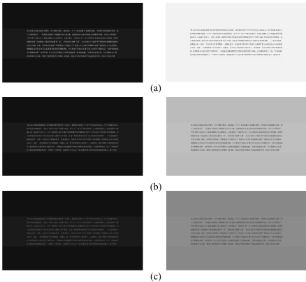
\includegraphics[width=\textwidth]{figures/luminance_contrast_1.png}
    \end{subfigure}
    \hfill % Separador d las dos imagenes
    % Segundo grupo (Derecho: d,e,f)
    \begin{subfigure}[b]{0.48\textwidth}
        \centering
        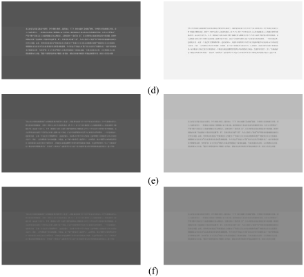
\includegraphics[width=\textwidth]{figures/luminance_contrast_2.png}
    \end{subfigure}
    
    \caption{Experimental Illustrations.}
    \label{fig:experimental_illustrations_all}
\end{figure}
\begin{figure}[H]
    \centering
    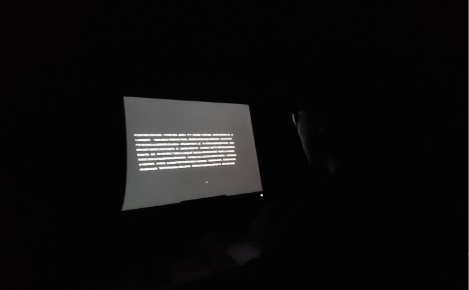
\includegraphics[width=0.8\textwidth]{figures/luminance_participation.png}
    \caption{Photo of participant during the experiment}
    \label{fig:luminance_participation}
\end{figure}


\subsection{The Effect of Display Polarity on Reading Speed and Reading Error Among Young Adults.\cite{Muhamad2024}}
\begin{table}[ht]   
    \centering
    \caption{Summary of the article by Muhamad and Mokhtar}
    \label{tab:muhamad2024}
    \begin{tabular}{|p{0.18\textwidth}|p{0.72\textwidth}|}
        \hline
        \textbf{Authors} & Muhamad, Nurulain \\
                         & Mokhtar, Nurliyana \\ \hline
        \textbf{Year}    & 2024 \\ \hline
        \textbf{Source}  & Journal of Health Science and Medical Research \\ \hline
        \textbf{DOI}     & \url{10.31584/jhsmr.20241095} \\ \hline
    \end{tabular}
\end{table}
\subsubsection{Reason for choice}
The reason for choosing this article is the fact that, even though the study is quite similar, they 
are not using an eye tracker but instead measuring times by hand, hence giving a general measurement 
with a lot of imprecisions. However, the methodology (without considering the tools for measuring) is 
an acceptable one, and some of it is considered while processing the data.

\begin{figure} [H]
    \centering
    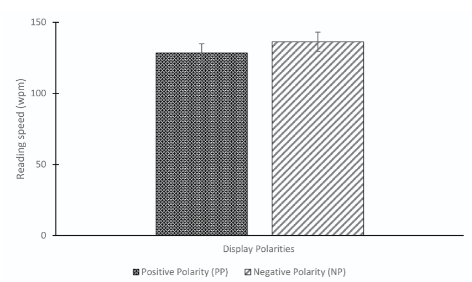
\includegraphics[width=0.8\textwidth]{figures/reading_speed_Muhamad.png}
    \caption{The comparison of reading speed between positive and negative display polarities.}
    \label{fig:reading_speed}
\end{figure}
Results:  
Reading speed, measured in words per minute (wpm), differed significantly between polarities, with negative 
polarity yielding higher speeds (136.27±25.58 wpm) compared to positive polarity (128.42±19.98 wpm), 
Z=-2.355, p-value\&lt;0.05. However, no significant polarity-related differences were found in reading errors, 
including mispronunciation (p-value=0.193) or omission (p-value=0.113).   Conclusion: Negative polarity 
displays enhanced reading performance by increasing reading speed; while reading errors remained unaffected.


\chapter{Hypothesis}
\label{chap:hypothesis}

\section{General Objective}
\section{Specific Objectives}
\section{Hypothesis}
The hypotheses to be proven in this thesis are:
\begin{enumerate}
    \item[H1)] Users using negative polarity are less fatigued than the positive polarity users
    \item[H2)] Users using negative polarity read quicker than positive polarity
    \item[H3)] Users prefer negative polarity over positive polarity
\end{enumerate}




\chapter{Methodology}
\label{chap:methodology}

\section{Experiment Design}
The experiment proposal is tightly attached to the idea of using an eye-tracking 
system, not only because it is an innovation that gives us more precision within 
the measurements but it also uniqueness surrounding the state of the art as really 
few experiments have used this device. To be more exact we will be using the eye 
tracking model Tobii Pro Nano\cite{tobii_pro_nano}. The experiment is briefly described 
in this section, but it will be further explained in the chapter \ref{chap:experiment_execution}.

The user will be prompted with a text message showing the instructions. 
This text comes along with a previous tobii calibration that will be further 
explained in the section \ref{sub:eye-tracker_calibration} and \ref{sub:user_instructions} respectively. 
 
After the instructions and calibration are completed, the second phase, 
the actual experiment can start. There are two possible paths, 
negative display polarity path or positive display polarity path. Both 
affect the instruction texts as long as the screenshots shown to the user. The 
wiki text was shown always the first being followed by the product description. 
The user has as much time as they want.  However, it wasn’t possible to return to 
previous pages.

Once the user finished reading the third phase would start, a questionnaire regarding
 preference will be shown, it also contains a small set of questions about the texts
  to ensure the user has been reading carefully. 

In addition, the webpages chosen for the experiment are \url{wikipedia.org} and \url{amazon.es}. 
These two webpages will be further explained in the \ref{sub:reading_task} section. 
\section{Population of Study}
In order to have a good experiment, not only is it important to have a consistent and well-prepared 
process but also have a focus population of study. The decision was to check for university students 
as this was the easiest and most accessible population given the situation. Therefore, the objective 
age was young people between 18 to 30 years old.

It is also worth mentioning that the objective was to find the usual user on the internet. For that 
an average user isn’t a computer scientist as they can be specialized on web design or other similar 
fields. This point made us go to the faculty of Economics as it was a larger faculty and the students 
can be considered an “average” user.

The objective was to have 80 persons in total 20 women and 20 men divided evenly between the negative 
and positive display polarity. However, due to the lack of collaboration of the people and the tendency
 to decline collaboration in the experiment, this was later reduced to 34 in total.

To summarize, it can be concluded that the conditions and population of the study were:
\begin{table}[ht]
    \centering
    \caption{Distribution of participants by gender, polarity, and age.}
    \label{tab:participants}
    \small
    \setlength{\tabcolsep}{3pt} % Distancia fija para todos
    % Formula generada por Gemini para tener una tabla así de guapa, ni idea de que significa esa linea
    \begin{tabularx}{\textwidth}{|>{\raggedright\arraybackslash}p{2.2cm}|*6{>{\centering\arraybackslash}X|}>{\centering\arraybackslash}p{1.2cm}|}
        \hline
        %Fila 1 y 1.5
        \multirow{2}{*}{\makecell{\textbf{Number of} \\ \textbf{partic.}}} & \multicolumn{2}{c|}{\makecell{\textit{Neg.} 
        \\ \textit{Pol.}}} & \multicolumn{2}{c|}{\makecell{\textit{Pos.} \\ \textit{Pol.}}} & \multicolumn{2}{c|}
        {\textbf{\textit{TOTAL}}} & \multirow{2}{*}{\textbf{\textit{Age}}} \\ \cline{2-7}  % Lo ultimo es para la edad y su respectivo separador
         & Obj. & Act. & Obj. & Act. & Obj. & Act. & \\ \hline
        % fila 2
        \textit{Men} & 20 & 7 & 20 & 7 & 40 & 14 & \multirow{2}{*}{\makecell{[18,30]}} \\ \cline{1-7}
        % Fila 3
        \textit{Women} & 20 & 10 & 20 & 10 & 40 & 20 & \\ \hline
        %fila 4
        \textbf{\textit{Total}} & 40 & 17 & 40 & 17 & 80 & 34 & \\ \hline
    \end{tabularx}
\end{table}

\section{Tools}
In order to accomplish the success of the experiment there is a need of some tools. 
They will be further explained why they are important ant what purpose do they serve. 
There is one hardware tool requirement and 3 software tools that are used to collect 
data and process it.
\subsection{Tobii Pro Nano}
The tobii pro nano it’s an eye-tracker currently discontinued by the owners (Tobii)\cite{tobii_pro_nano} 
that is still to its day a great tool to collect user data. It’s worth mentioning that this 
tool is quite expensive and to use it the University of Oviedo has lent me one unit. Always
 with the surveillance of my tutors. The tobii pro nano is the lightest and most portable 
 unit offered, however it has some limitations that won’t be a problem in our case as the 
 limitations are for precise operations. 
 \begin{figure}
    \centering
    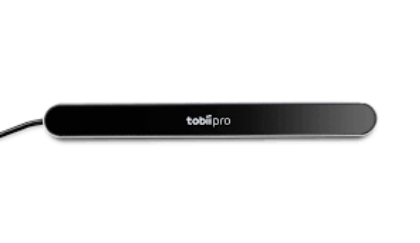
\includegraphics[width=0.5\textwidth]{figures/tobii_pro_nano.png}
    \caption{Tobii Pro Nano Device\cite{tobii_pro_nano}}
 \end{figure}
\subsubsection{Eye Tracker Technology Breakdown}
The eye tracker works in an amazing way, the process is a combination of high-quality cameras. 
Using what’s commonly called Pupil Center Corneal Reflection (PCCR). In the case of tobii pro 
nano it uses a patented variant of PCCR (US Patent US7,572,008).\cite{How_do_eyetrackers_work}

The PCCR is a mix between “illuminators” that is components that are almost infrared sensors 
that create such light on the eyes. Then different sets of cameras take pictures of the eye 
patterns and reflections. That is sent to algorithms that detect those patterns and reflections
 creating a detailed 3D model of the eye position and its gazes \cite{How_do_eyetrackers_work}.

\subsection{Tobii Pro Lab}
\begin{figure} [htb]
    \centering
    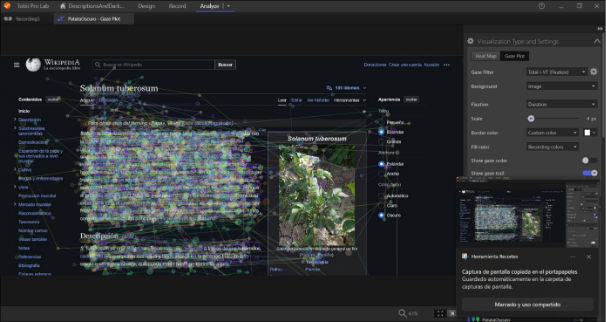
\includegraphics[width=0.5\textwidth]{figures/tobii_pro_lab.png}
    \caption{Tobii Pro Lab Software\cite{tobii_pro_lab}}
\end{figure}
The eye-tracking device connects to a software application called “Tobii Pro Lab”. This 
application aims to ease the use, collection and analysis of the gaze data. Curiously this is
 a negative display polarity program. It is needed to have a license in order to use it. 
 However, a 30 day trial is provided which has been enough toextract the data, change or create 
 the desired data, download it and process it. The data was gathered in the laptop of my proffesor
  as they have the paid license.Some of the most interesting tools are the visualization of heat maps, 
  recordings and the Areas of Interest, that will be further explained.

\subsection{Google Forms}
Google Forms is a free tool developed by Google that allows google users to create forms. This is a 
powerful tool as the answers can be stored in a Google Spreadsheet that can be exported as a .csv 
archive to be later processed. This tool is also pretty compatible with the tobii pro lab when creating 
the timelines that the user is going to be exposed due to the fact of the possibility of running.
\begin{figure}
    \centering
    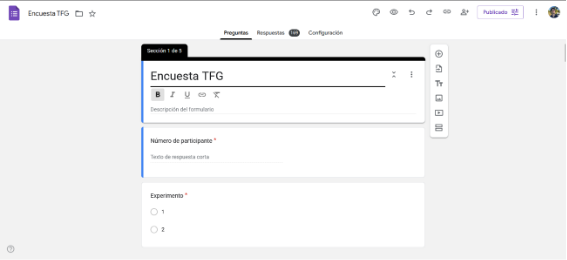
\includegraphics[width=0.5\textwidth]{figures/google_forms_example.png}
    \caption{Google Forms Example}
\end{figure}
\subsection{Python 3}
There’re few programming languages that almost everyone on earth has heard of, this is the case.
 Python is a powerful programming language not because of its speed or performance but because of
  the libraries that are available. This python environment makes room to one of the biggest spaces 
  for data processing. In my case, I’m not a specialized student on data processing, that’s why a 
  well-known and big space like this can be the perfect tool to approach a thesis. 
\subsubsection{Python external libraries}
As mentioned beforehand, the prowess of python resides in its libraries. The libraries used for this thesis are:
\begin{itemize}
    \item \textbf{Pandas}\cite{pandas}: Pandas is a library centered around the idea of easing
    data manipulation and analysis by providing a generic data structure called DataFrame. It is 
    almost an standard in the data ecosystem of python.
    \item \textbf{Matplotlib}\cite{matplotlib}: Matplotlib strength resides in its flexibility to 
    create any kind of graph. It is one of the most used libraries in Python.
    \item \textbf{NumPy}\cite{numpy}: NumPy name comes from “Numerical Python” and it is a library that provides 
    aid for the manipulation of arrays of data. It combines pretty well with Pandas as every column or row of a
    DataFrame can be transformed into a NumPy array easily.
    \item \textbf{SciPy}\cite{scipy}: SciPy is a library created for scientific and technical computing.
    Providing a large amount of functions for many different fields. In the case of this study, the biggest use
    resided in the statistics algorithms like Mann-Whitney U test and the t-test.
  \end{itemize}

\subsection{Dark Reader}
Given that the objective is to analyze the effects of display polarity on texts the decision was to
 choose a wiki page as it is a tool that until this day many users do. Moreover, an e-commerce is 
 another safe bet. In order to make it the most average the decision was to use “wikiedia.org” and
  “amazon.es”. However, the e-commerce website didn’t allow negative polarity, so we had to use a 
  firefox extension called Dark Reader which you can see in figure \ref{fig:dark_reader}

  \begin{figure}
    \centering
    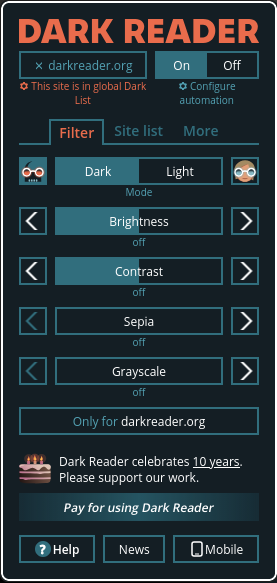
\includegraphics[width=0.5\textwidth]{figures/dark_reader.png}
    \caption{Dark Reader Extension\cite{dark_reader}}
    \label{fig:dark_reader}
  \end{figure}

\subsection{Python Web Interaction Behaviour (Pywib)}


Pywib\cite{clicks} is a python library desgined for the analysis of user behaviour within webpages. 
This library is still in development by a colleague of mine called Guillermo Dylan Carvajal and
despite of this tool is still in early stages, it is strong enough to be used in the analysis of this study.

TODO: Añadir más info sobre que funciones se han usado y para que sirven.
\chapter{Experiment Execution}
\label{chap:experiment_execution}

\section{Environmental Conditions}
The experiment was developed in the Faculty of Economics of the University of Oviedo, 
located in the city of Oviedo during the 23rd and 25th of April. The weather was cloudy 
with few intermittent rains, this led to a general dim light. In order to have proper 
lighting and stable conditions the room was illuminated with fluorescent lights giving a 
total of 7,2 Exposure Value (EV) on the first day and 7,3 EV the second day.

Regarding the placement of the experiment, we were in a Main Hall in the calmest possible 
place. Experiment subjects would sit in a chair with a small table holding the laptop and 
the eye-tracker. The average distance between the experiment subjects and the screen was 
60 cm as suggested by the tobii pro lab.

\section{Experiment Phases}
\label{sec:experiment_phases}
The first and most 3 phase of the experiment consisted of a tobii calibration. As this is a
 key factor and it was desired to have a lot of precision during the experiment, that is why 
 the 9-point calibration was chosen. Experiment subjects were asked to watch and follow a 
 white dot on the screen after this was finished the calibration results were shown. In the 
 case the results were favorable the experiment would continue or else the calibration would 
 be repeated entirely or partially.

\subsection{Eye-tracker Calibration}
\label{sub:eye-tracker_calibration}
The second phase of the experiment already had two different versions. One consisted of the 
instructions displayed in negative polarity and the other one prompted the instructions in 
positive polarity. Results of this have been recorded but not taken into account inside the 
experiment as they are outside of the aim of web based texts.

\subsection{User Instructions}
\label{sub:user_instructions}
\subsection{Reading Task}
\label{sub:reading_task}
The reading task consisted of 2 texts. The first texts is based on Wikipedia newest negative 
and positive display polarity while the first text is based on Amazon web-page along with the 
plugin “Dark Reader” explained above in the document. The pages displayed were centered around 
daily objects with complex enough information so It wouldn’t be a technical hurdle while not 
being too simple to read. 

\subsubsection{Wikipedia article}
The chosen Wikipedia page refers to such a common food as the potato A CONTINUAR AQUI!!!!!!!!!!!!!!!!!!!!
\begin{figure}
    \centering
    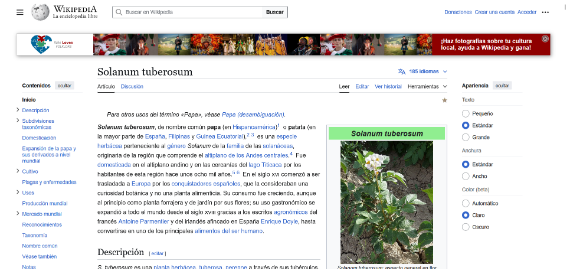
\includegraphics[width=0.8\textwidth]{figures/patata_claro.png}
    \caption{Wikipedia page about potatoes in positive display polarity\cite{patata}}
    \label{fig:patata_claro}
\end{figure}
\begin{figure}
    \centering
    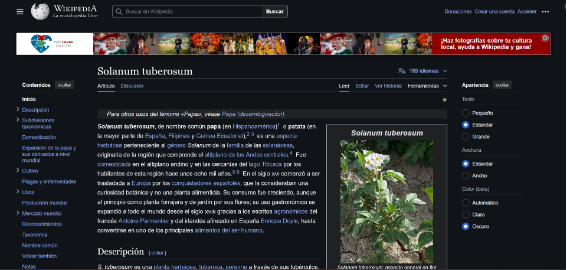
\includegraphics[width=0.8\textwidth]{figures/patata_oscuro.png}
    \caption{Wikipedia page about potatoes in negative display polarity\cite{patata}}
    \label{fig:patata_oscuro}
\end{figure}

\subsubsection{Amazon product}
\begin{figure}
    \centering
    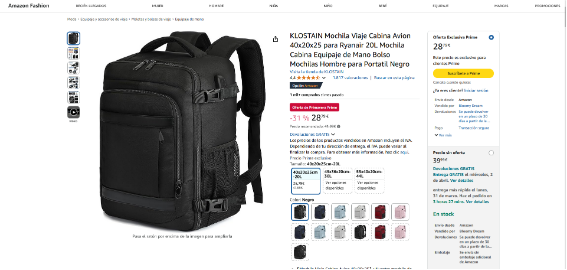
\includegraphics[width=0.8\textwidth]{figures/mochila_claro.png}
    \caption{Amazon product page in positive display polarity\cite{mochila}}
    \label{fig:amazon_claro}
\end{figure}
\begin{figure}
    \centering
    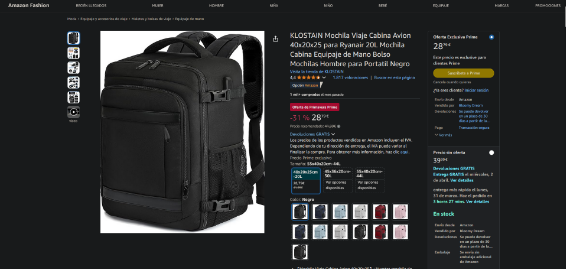
\includegraphics[width=0.8\textwidth]{figures/mochila_oscuro.png}
    \caption{Amazon product page in negative display polarity\cite{mochila}}
    \label{fig:amazon_oscuro}
\end{figure}
\subsection{Final Questionnaire}
\chapter{Data Analysis}
\label{chap:data_analysis}

\section{Data Preprocessing}
\section{Chosen Metrics}
\section{Statistical Analysis Methods}
\chapter{Results}
\label{chap:results}
\section{Eye-traker Data}
The study developed in python has proven interesting results regarding the 
metrics mentioned in chapter \ref{chap:data_analysis}. The results will show the results of the statistics along with
the basic statistical values such as mean and standard deviation.
\subsection{Total Duration of Whole Fixations}
Table \ref{tab:tdwf_basic_stats} shows that the mean was higher in length for positive polarity in all TOIs,
having the biggest difference in the Wiki-Based Scene.
\begin{table}[H]
    \centering
    \small
    \setlength{\tabcolsep}{4pt}
    \renewcommand{\arraystretch}{1.3}
    \caption{Results of Total Duration of Whole Fixations}
    \label{tab:tdwf_basic_stats}

    \resizebox{0.98\linewidth}{!}{
    \begin{tabular}{|c|c|c|c|c|c|}
        \hline
        \textbf{Display Polarity} & \textbf{TOI} & \shortstack{\textbf{Min.} \\ \textbf{(ms)}} & \shortstack{\textbf{Mean} \\ \textbf{(ms)}} & \shortstack{\textbf{Std.} \\ \textbf{Deviation} \\ \textbf{(ms)}} & \shortstack{\textbf{Max.} \\ \textbf{(ms)}} \\ \hline
        

        \multirow{3}{*}{Positive Polarity} & \textbf{Wiki-based} & 18570 & 52902.88 & 24410.26 & 125026 \\ \cline{2-6}
         & \textbf{E-Commerce} & 9443 & 64217.12 & 34024.20 & 125642 \\ \cline{2-6}
         & \textbf{Entire Exp.} & 215011 & 347509 & 81449.08 & 504168 \\ \hline
        

        \multirow{3}{*}{Negative Polarity} & \textbf{Wiki-based} & 2631 & 41879.59 & 17204.72 & 72631 \\ \cline{2-6}
         & \textbf{E-Commerce} & 8977 & 53989.41 & 22480.35 & 94915 \\ \cline{2-6}
         & \textbf{Entire Exp.} & 154088 & 282626.65 & 63197.95 & 391933 \\ \hline
    \end{tabular}
    }
\end{table}
Figure \ref{fig:tdwf_boxplot} shows how only the entire experiment has significant results within this variable. 
Further statistics can be seen in table \ref{tab:tdwf_stats} where p-values under $\alpha=0.05$ are highlighted in 
red and p-values under $\alpha=0.1$ are highlighted in orange. 
\begin{figure}[H]
    \centering
    \includegraphics[width=0.8\textwidth]{figures/Total_Duration_of_Whole_Fixations.png}
    \caption{Total Duration of Fixations for each Display Polarity and TOI.}
    \label{fig:tdwf_boxplot}
\end{figure}

\begin{table}[H]
    \centering
    \small
    \setlength{\tabcolsep}{4pt}
    \caption{Statistics of Total Duration of Whole Fixations}
    \label{tab:tdwf_stats}
    \resizebox{0.98\linewidth}{!}{
    \begin{tabular}{|c|c|c|c|c|}
        \hline
        \textbf{TOI} & \textbf{W\textsubscript{PP}} & \textbf{W\textsubscript{NP}} & \textbf{T-Student} & \textbf{Mann-Whitney} \\ \hline
        Wiki-Based & \textbf{\color{red}0.0091} & 0.7774 & - & 0.2557 \\ \hline
        E-Commerce & 0.7094 & 0.9138 & 0.3244 & - \\ \hline
        Entire Exp. & 0.8348 & 0.9790 & \textbf{\color{red}0.0174} & - \\ \hline
    \end{tabular}
    }
\end{table}

\subsection{Total Number of Fixations}
Regarding the total number of fixations, table \ref{tab:tnf_basic_stats} proves that the mean number of fixations 
is higher in positive polarity in every single TOI.
\begin{table}[H]
    \centering
    \small
    \setlength{\tabcolsep}{4pt}
    \renewcommand{\arraystretch}{1.3}
    \caption{Results of Total Number of Fixations}
    \label{tab:tnf_basic_stats}

    \resizebox{0.98\linewidth}{!}{
    \begin{tabular}{|c|c|c|c|c|c|}
        \hline
        \textbf{Display Polarity} & \textbf{TOI} & \shortstack{\textbf{Min.}} & \shortstack{\textbf{Mean}} & \shortstack{\textbf{Std.} \\ \textbf{Deviation}} & \shortstack{\textbf{Max.}} \\ \hline
        

        \multirow{3}{*}{Positive Polarity} & \textbf{Wiki-based} & 62 & 158.94 & 52.41 & 301 \\ \cline{2-6}
         & \textbf{E-Commerce} & 35 & 199.06 & 92.76 & 320 \\ \cline{2-6}
         & \textbf{Entire Exp.} & 545 & 979.59 & 240.28 & 1510 \\ \hline
        

        \multirow{3}{*}{Negative Polarity} & \textbf{Wiki-based} & 13 & 142.65 & 50.59 & 208 \\ \cline{2-6}
         & \textbf{E-Commerce} & 45 & 194.06 & 64.46 & 280 \\ \cline{2-6}
         & \textbf{Entire Exp.} & 405 & 844.82 & 162.51 & 1159\\ \hline
    \end{tabular}
    }
\end{table}
The statistical analysis, as seen in figure \ref{fig:tnf_boxplot} and table \ref{tab:tnf_stats}. There is no
significant difference between both groups but the entire experiment is close to be significant with a p-value of 0.0736 in the T-Student test.
\begin{figure}[H]
    \centering
    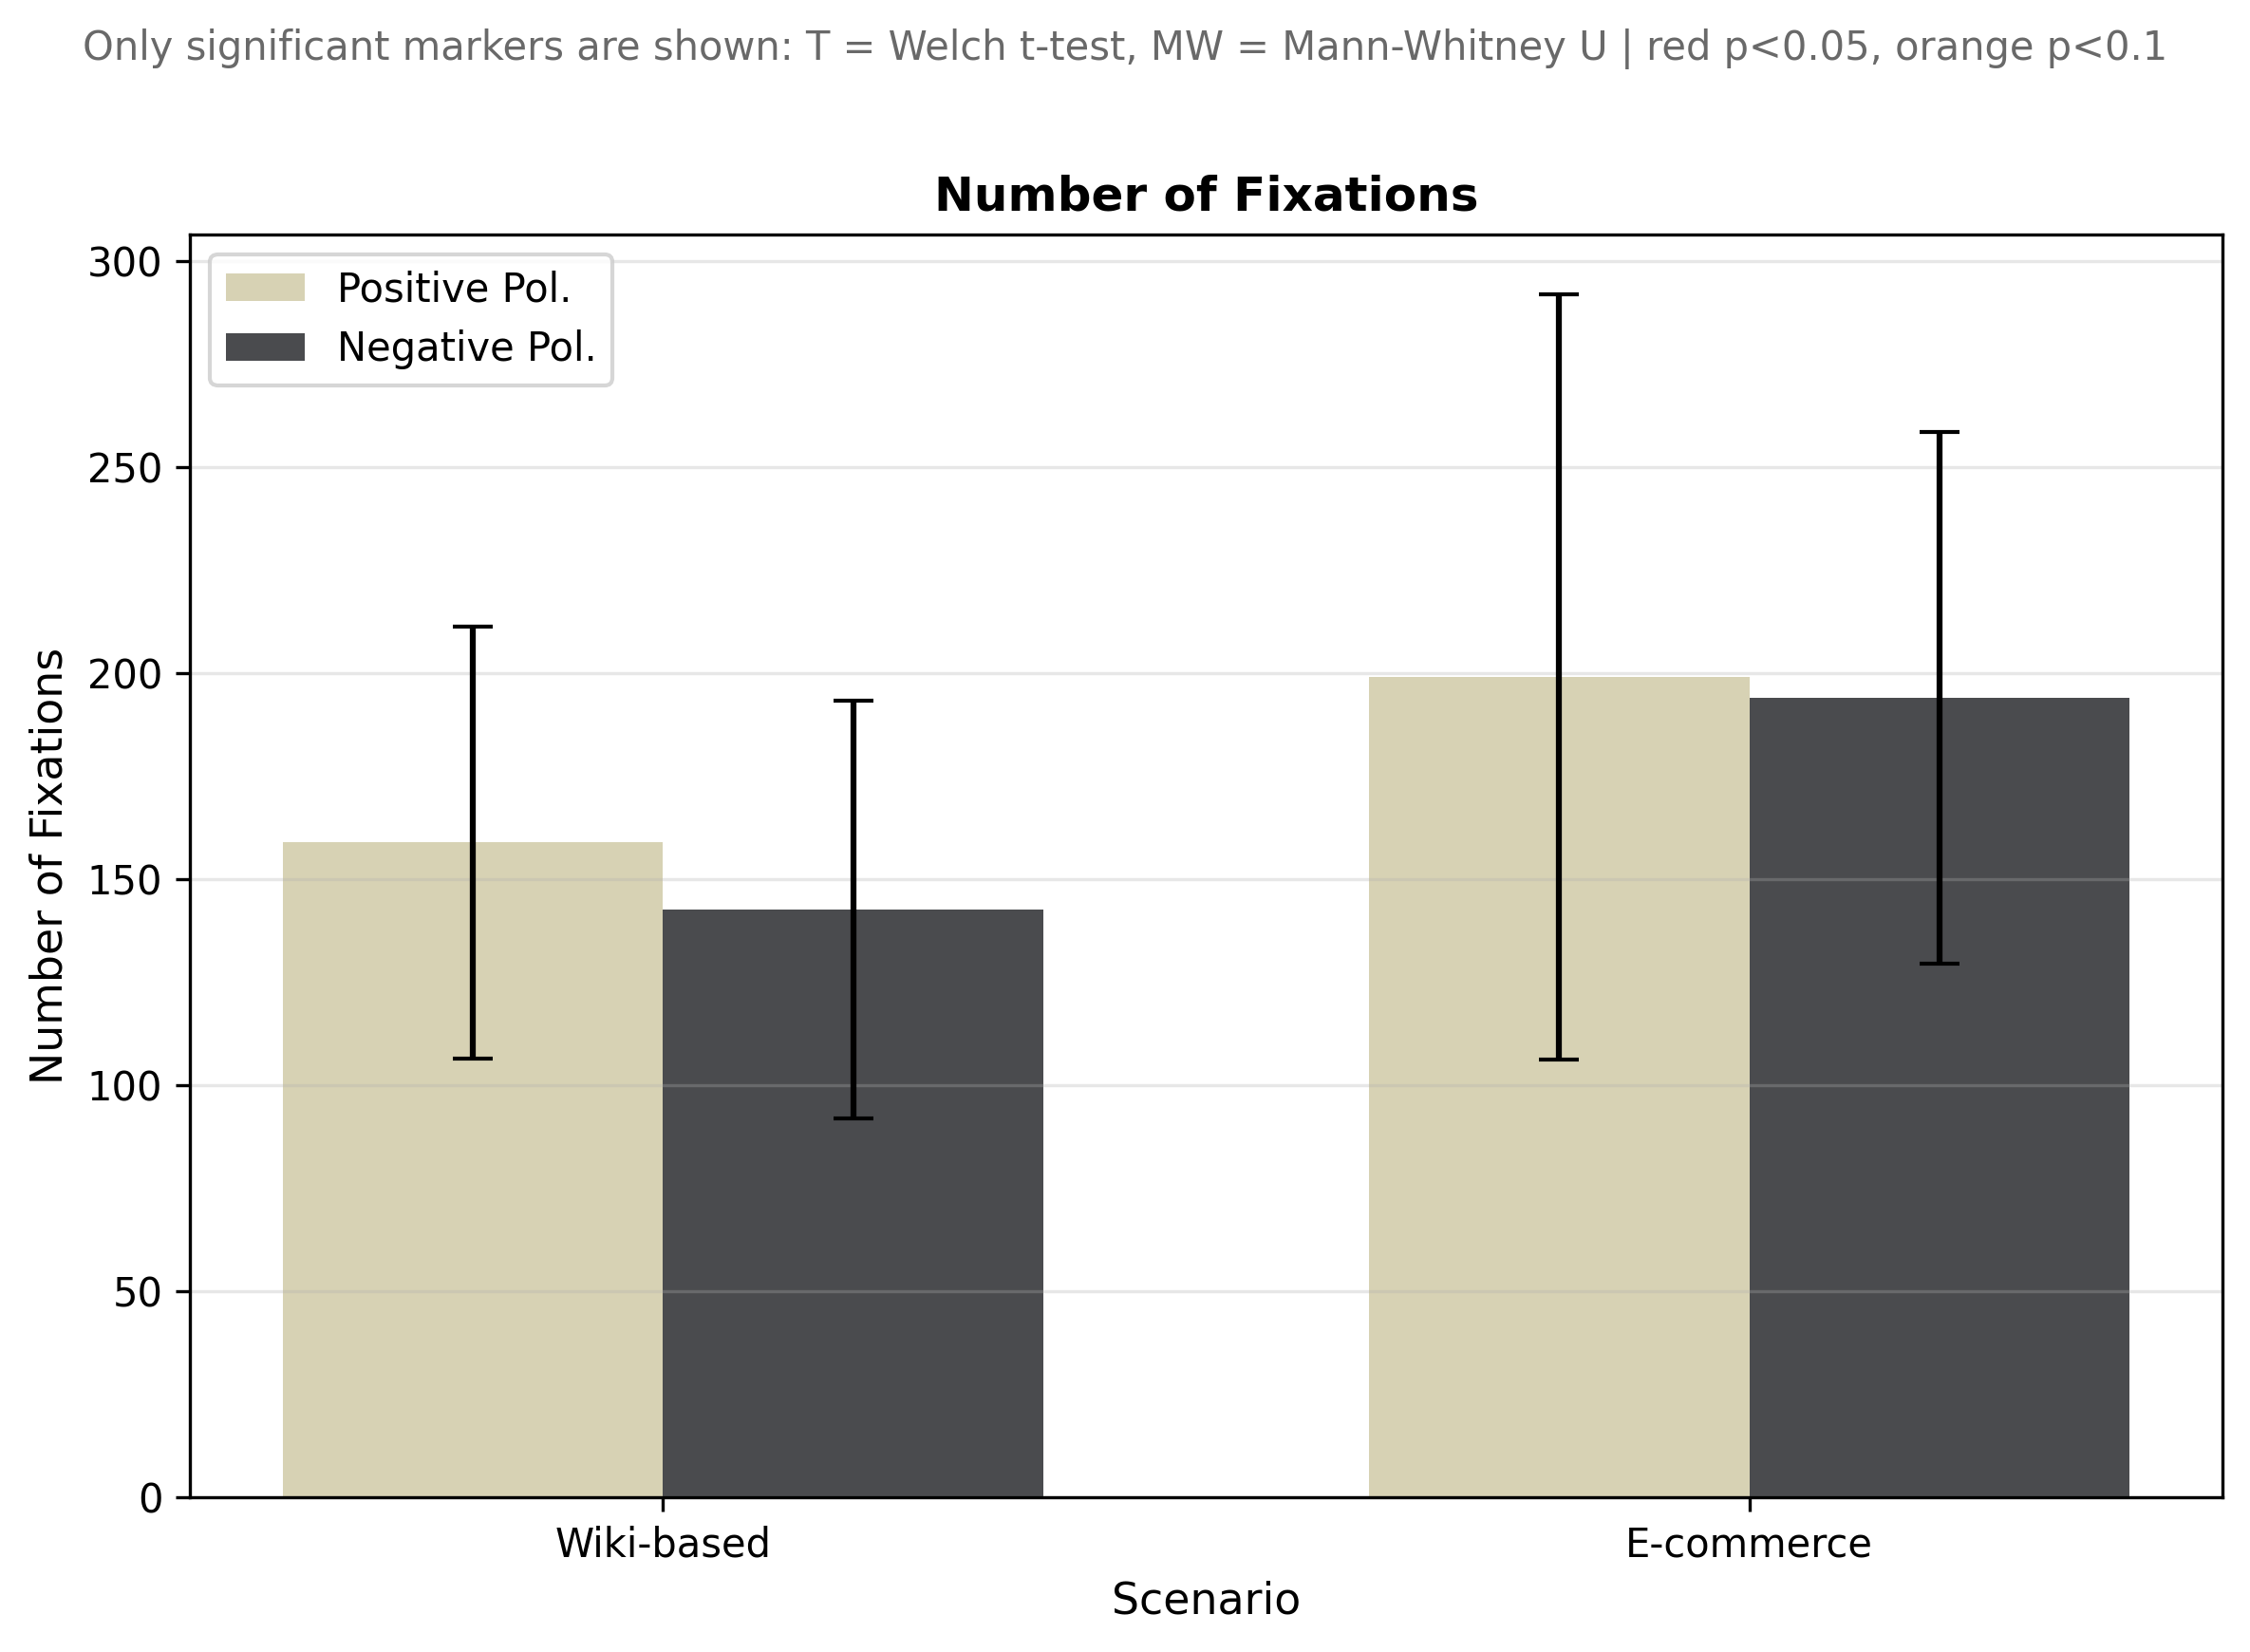
\includegraphics[width=0.8\textwidth]{figures/Number_of_whole_fixations.png}
    \caption{Total Number of Fixations for each Display Polarity and TOI.}
    \label{fig:tnf_boxplot}
\end{figure}

\begin{table}[H]
    \centering
    \small
    \setlength{\tabcolsep}{4pt}
    \caption{Statistics of Total Number of Fixations}
    \label{tab:tnf_stats}
    \resizebox{0.98\linewidth}{!}{
    \begin{tabular}{|c|c|c|c|c|}
        \hline
        \textbf{TOI} & \textbf{W\textsubscript{PP}} & \textbf{W\textsubscript{NP}} & \textbf{T-Student} & \textbf{Mann-Whitney} \\ \hline
        Wiki-Based & 0.5150 & 0.2003 & 0.3776 & - \\ \hline
        E-Commerce & 0.1019 & 0.1089 & 0.8591 & - \\ \hline
        Entire Exp. & 0.5321 & 0.3570 & \textbf{\color{orange}0.0736} & - \\ \hline
    \end{tabular}
    }
\end{table}

\subsection{Duration of First Fixation}
The first duration of fixation is lower in positive polarity in both TOIS but differs in the whole recording,
as shown in table \ref{tab:dfff_basic_stats}. 
\begin{table}[H]
    \centering
    \small
    \setlength{\tabcolsep}{4pt}
    \renewcommand{\arraystretch}{1.3}
    \caption{Results of Duration of First Fixation}
    \label{tab:dfff_basic_stats}

    \resizebox{0.98\linewidth}{!}{
    \begin{tabular}{|c|c|c|c|c|c|}
        \hline
        \textbf{Display Polarity} & \textbf{TOI} & \shortstack{\textbf{Min.} \\ \textbf{(ms)}} & \shortstack{\textbf{Mean} \\ \textbf{(ms)}} & \shortstack{\textbf{Std.} \\ \textbf{Deviation} \\ \textbf{(ms)}} & \shortstack{\textbf{Max.} \\ \textbf{(ms)}} \\ \hline
        

        \multirow{3}{*}{Positive Polarity} & \textbf{Wiki-based} & 83 & 181.21 & 111.99 & 583 \\ \cline{2-6}
         & \textbf{E-Commerce} & 133 & 193 & 54.03 & 316 \\ \cline{2-6}
         & \textbf{Entire Exp.} & 67 & 315.47 & 268.45 & 1016 \\ \hline
        

        \multirow{3}{*}{Negative Polarity} & \textbf{Wiki-based} & 100 & 205.82 & 100.07 & 533 \\ \cline{2-6}
         & \textbf{E-Commerce} & 83 & 200 & 123.55 & 650 \\ \cline{2-6}
         & \textbf{Entire Exp.} & 67 & 203.88 & 163.85 & 766 \\ \hline
    \end{tabular}
    }
\end{table}
\begin{figure}[H]
    \centering
    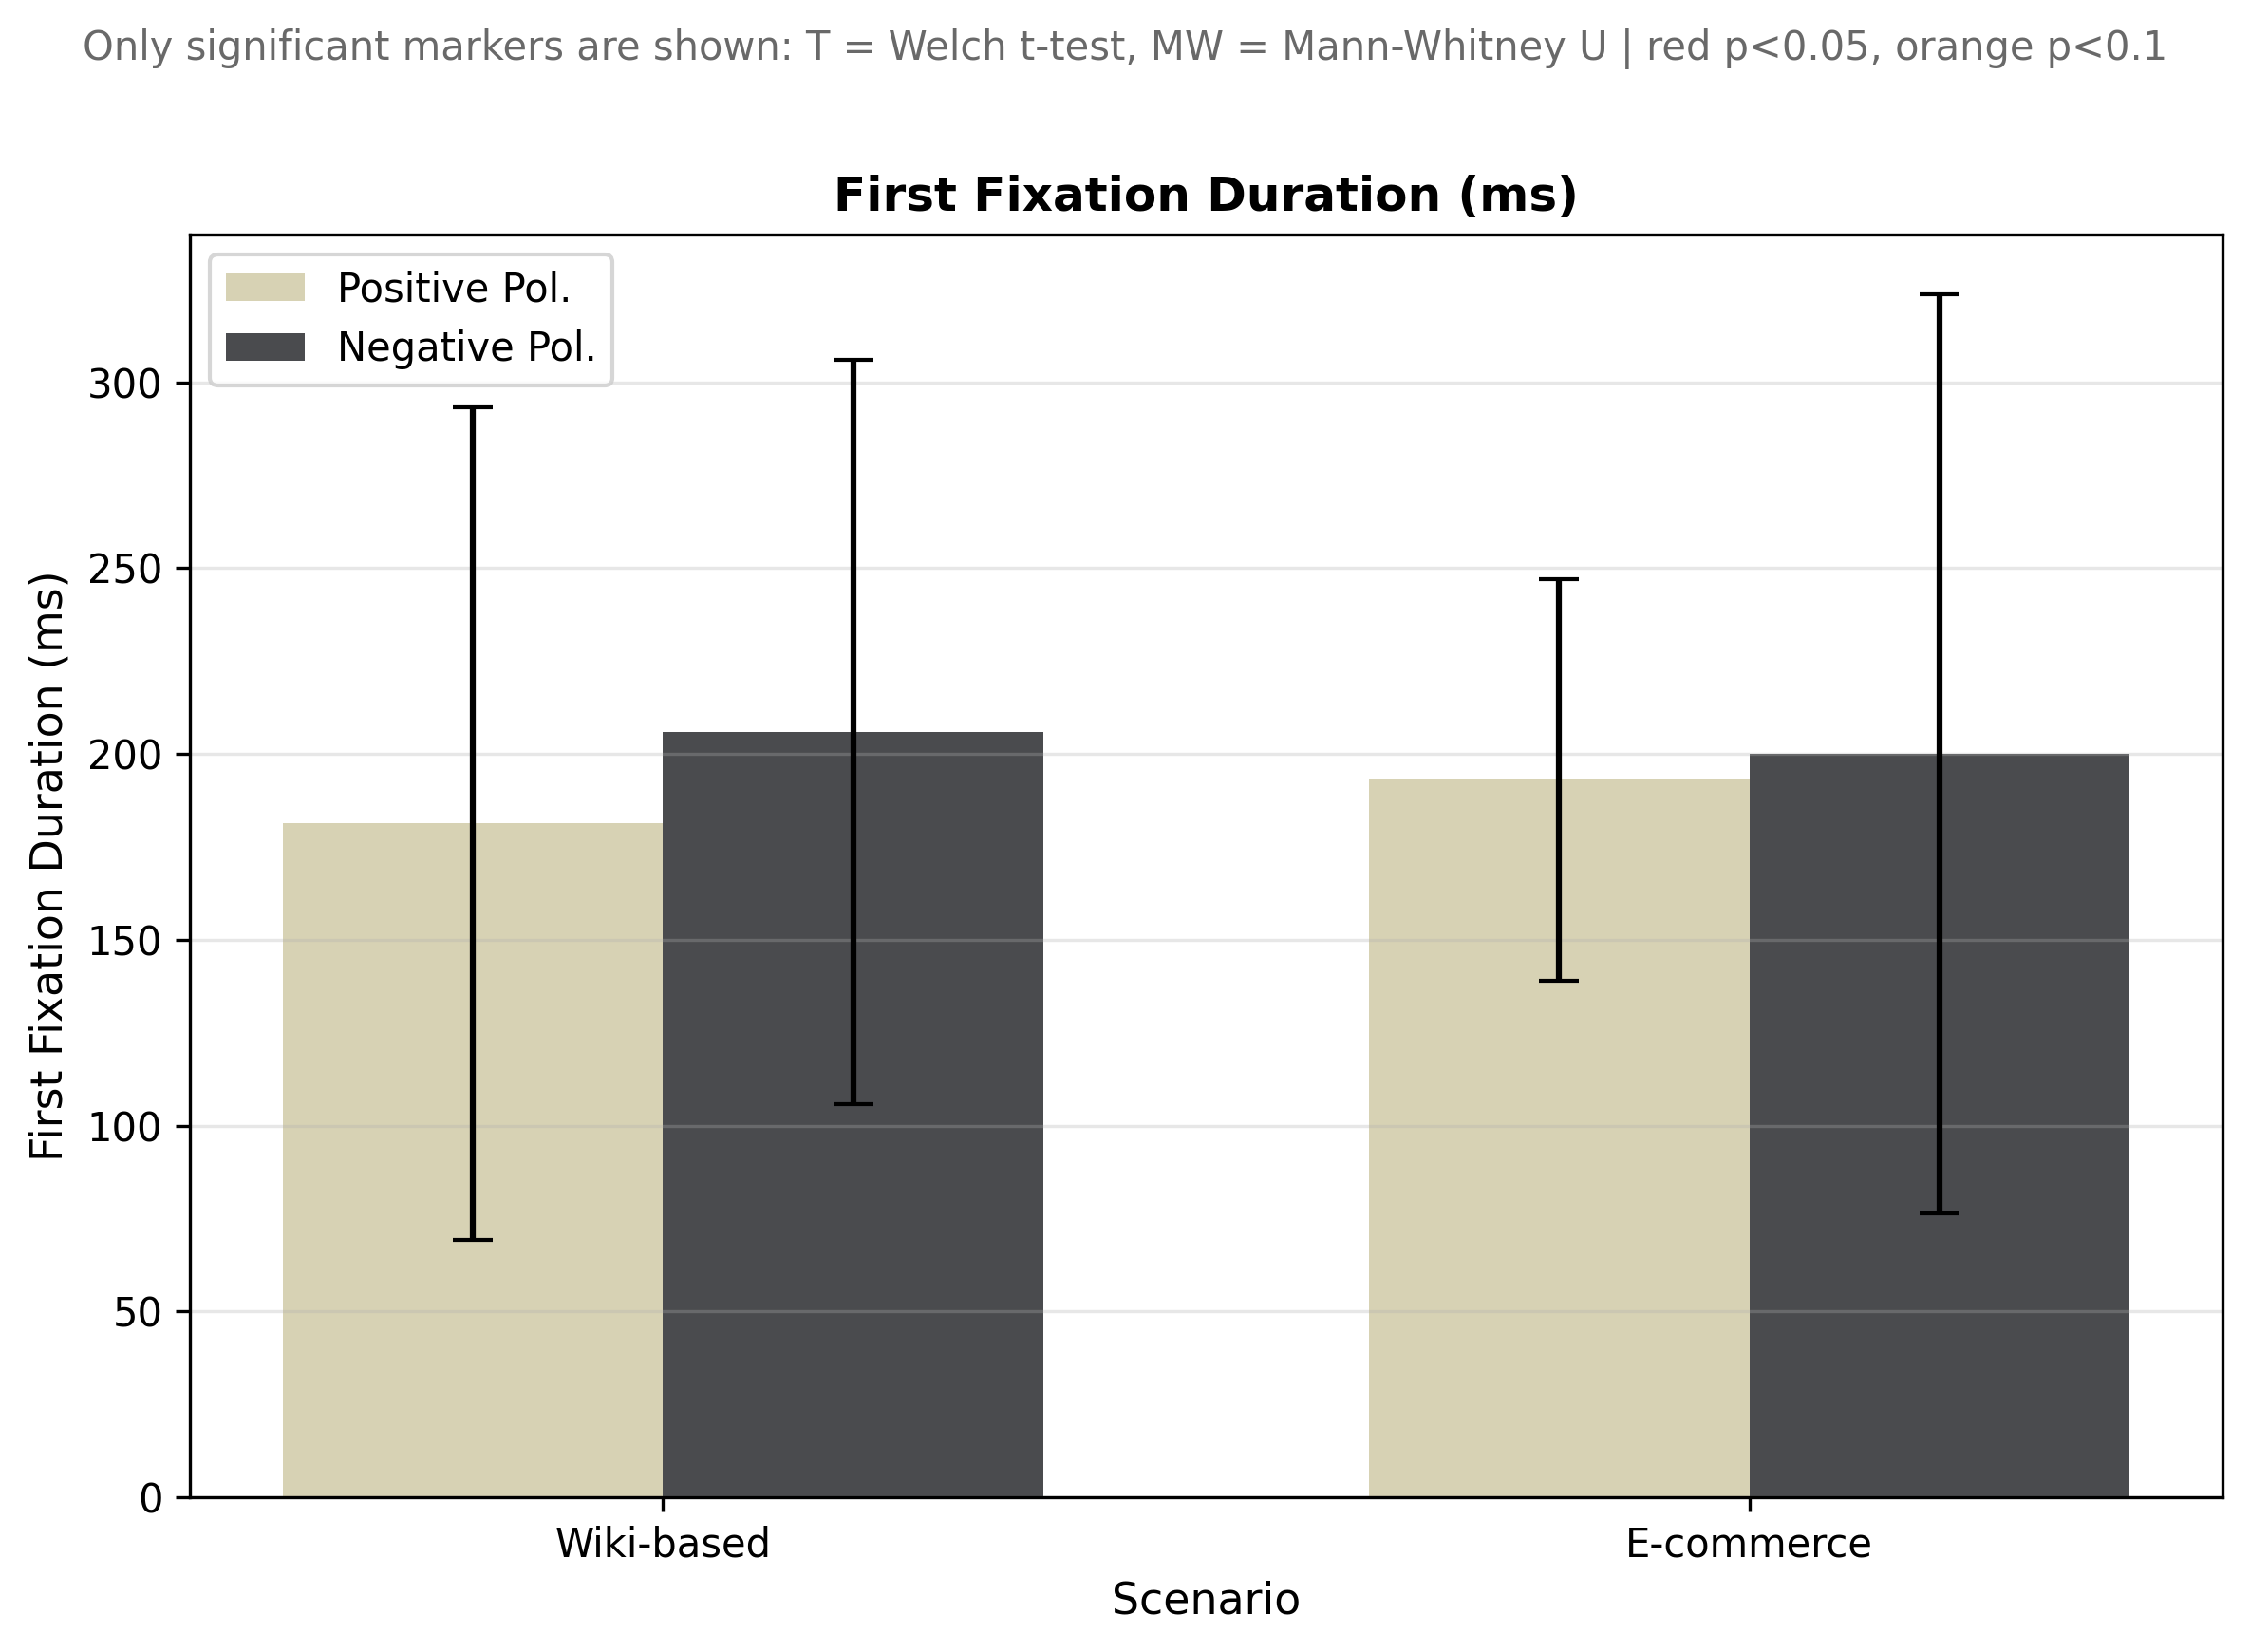
\includegraphics[width=0.8\textwidth]{figures/Duration_of_first_whole_fixation.png}
    \caption{Duration of First Fixation for each Display Polarity and TOI.}
    \label{fig:dfff_boxplot}
\end{figure}
The statistical analysis in this case shows how none of the TOIS follows a normal distribution, as shown in table
\ref{tab:dfff_stats} resulting in the Mann-Whitney U test where none of the TOIS is significant, see figure \ref{fig:dfff_boxplot}.
\begin{table}[H]
    \centering
    \small
    \setlength{\tabcolsep}{4pt}
    \caption{Statistics of Duration of First Fixation}
    \label{tab:dfff_stats}
    \resizebox{0.98\linewidth}{!}{
    \begin{tabular}{|c|c|c|c|c|}
        \hline
        \textbf{TOI} & \textbf{W\textsubscript{PP}} & \textbf{W\textsubscript{NP}} & \textbf{T-Student} & \textbf{Mann-Whitney} \\ \hline
        Wiki-Based & \textbf{\color{red}0.0001} & \textbf{\color{red}0.0005} & - & 0.3224 \\ \hline
        E-Commerce & \textbf{\color{red}0.0048} & \textbf{\color{red}0.0000} & - & 0.5434 \\ \hline
        Entire Exp. & \textbf{\color{red}0.0046} & \textbf{\color{red}0.0002} & - & 0.3005 \\ \hline
    \end{tabular}
    }
\end{table}

\subsection{Average Duration of Fixations}
The average duration of fixations seems to be higher in positive polarity in every single TOI, as shown in table
\ref{tab:adf_basic_stats}. This difference is more steep in the Wiki-Based scene.
\begin{table}[H]
    \centering
    \small
    \setlength{\tabcolsep}{4pt}
    \renewcommand{\arraystretch}{1.3}
    \caption{Results of Average Duration of Fixations}
    \label{tab:adf_basic_stats}

    \resizebox{0.98\linewidth}{!}{
    \begin{tabular}{|c|c|c|c|c|c|}
        \hline
        \textbf{Display Polarity} & \textbf{TOI} & \shortstack{\textbf{Min.} \\ \textbf{(ms)}} & \shortstack{\textbf{Mean} \\ \textbf{(ms)}} & \shortstack{\textbf{Std.} \\ \textbf{Deviation} \\ \textbf{(ms)}} & \shortstack{\textbf{Max.} \\ \textbf{(ms)}} \\ \hline
        

        \multirow{3}{*}{Positive Polarity} & \textbf{Wiki-based} & 234 & 329.29 & 79.39 & 537 \\ \cline{2-6}
         & \textbf{E-Commerce} & 236 & 318.41 & 63.58 & 457 \\ \cline{2-6}
         & \textbf{Entire Exp.} & 288 & 358.88 & 43.08 & 451 \\ \hline
        

        \multirow{3}{*}{Negative Polarity} & \textbf{Wiki-based} & 202 & 287.53 & 57.97 & 441 \\ \cline{2-6}
         & \textbf{E-Commerce} & 193 & 272.19 & 58.81 & 407 \\ \cline{2-6}
         & \textbf{Entire Exp.} & 262 & 336.18 & 46.65 & 436 \\ \hline
    \end{tabular}
    }
\end{table}
Regarding the statistical analysis, only a relevant result exists for the E-Commerce scene with the p-value of 0.0514 
being pretty close to the significance level.
\begin{figure}[H]
    \centering
    \includegraphics[width=0.8\textwidth]{figures/Average_Duration_of_whole_fixations.png}
    \caption{Average Duration of Fixations for each Display Polarity and TOI.}
    \label{fig:adf_boxplot}
\end{figure}
\begin{table}[H]
    \centering
    \small
    \setlength{\tabcolsep}{4pt}
    \caption{Statistics of Average Duration of Fixations}
    \label{tab:adf_stats}
    \resizebox{0.98\linewidth}{!}{
    \begin{tabular}{|c|c|c|c|c|}
        \hline
        \textbf{TOI} & \textbf{W\textsubscript{PP}} & \textbf{W\textsubscript{NP}} & \textbf{T-Student} & \textbf{Mann-Whitney} \\ \hline
        Wiki-Based & \textbf{\color{red}0.0365} & 0.2901 & - & 0.1528 \\ \hline
        E-Commerce & \textbf{\color{red}0.0200} & 0.4693 & - & \textbf{\color{orange}0.0514} \\ \hline
        Entire Exp. & 0.6286 & 0.8766 & 0.1624 & - \\ \hline
    \end{tabular}
    }
\end{table}

\subsection{Average Peak Velocity}
The average peak velocity is higher in negative polarity for every TOI as seen in table \ref{tab:apv_basic_stats}. However, 
It is only relevant in the entire recording with a p-value of 0.0871 proven in table \ref{tab:apv_stats} and figure \ref{fig:aspv_boxplot}
\begin{table}[H]
    \centering
    \small
    \setlength{\tabcolsep}{4pt}
    \renewcommand{\arraystretch}{1.3}
    \caption{Results of Average Peak Velocity}
    \label{tab:apv_basic_stats}

    \resizebox{0.98\linewidth}{!}{
    \begin{tabular}{|c|c|c|c|c|c|}
        \hline
        \textbf{Display Polarity} & \textbf{TOI} & \shortstack{\textbf{Min.} \\ \textbf{(º/s)}} & \shortstack{\textbf{Mean} \\ \textbf{(º/s)}} & \shortstack{\textbf{Std.} \\ \textbf{Deviation} \\ \textbf{(º/s)}} & \shortstack{\textbf{Max.} \\ \textbf{(º/s)}} \\ \hline
        

        \multirow{3}{*}{Positive Polarity} & \textbf{Wiki-based} & 89.13 & 107.76 & 15.84 & 148.82 \\ \cline{2-6}
         & \textbf{E-Commerce} & 77.19 & 102.25 & 24.92 & 189.92 \\ \cline{2-6}
         & \textbf{Entire Exp.} & 91.69 & 106.49 & 7.09 & 119.99 \\ \hline
        

        \multirow{3}{*}{Negative Polarity} & \textbf{Wiki-based} & 79.57 & 118.72 & 29.61 & 216.31 \\ \cline{2-6}
         & \textbf{E-Commerce} & 76.66 & 104.02 & 16.63 & 133.35 \\ \cline{2-6}
         & \textbf{Entire Exp.} & 88.48 & 112.61 & 11.79 & 135.44 \\ \hline
    \end{tabular}
    }
\end{table}
\begin{figure}[H]
    \centering
    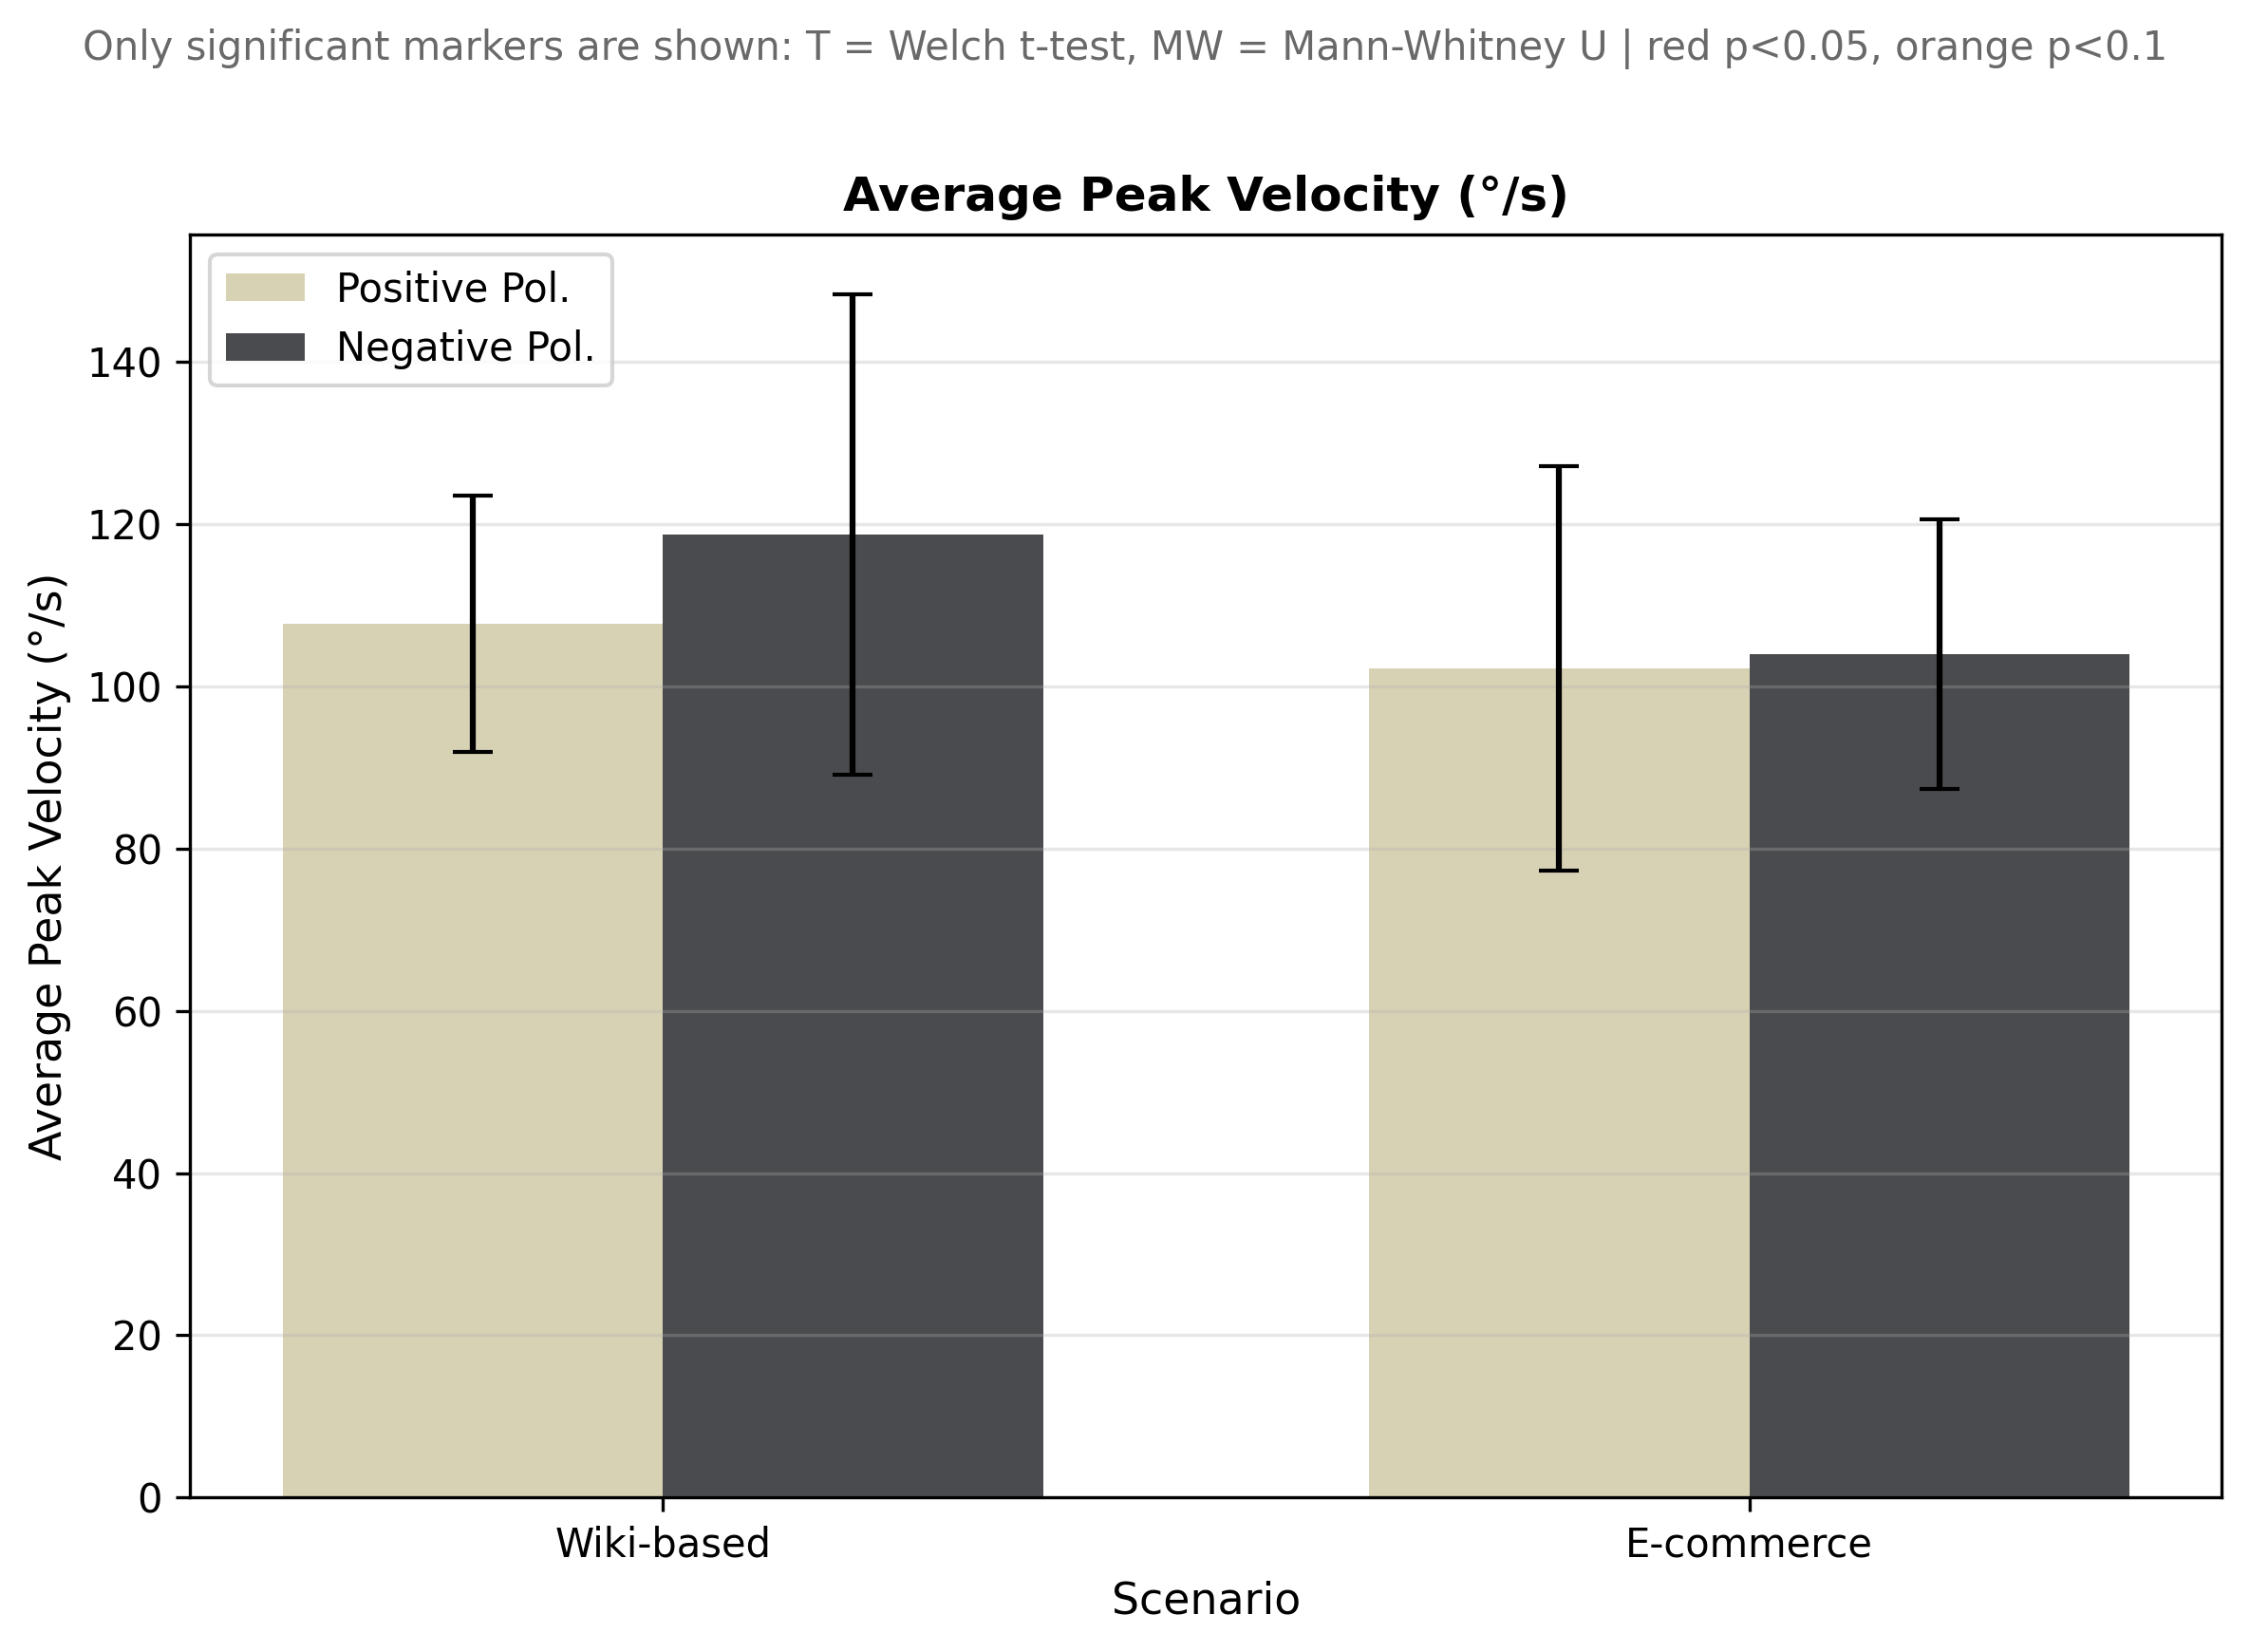
\includegraphics[width=0.8\textwidth]{figures/Average_peak_velocity_of_saccades.png}
    \caption{Average Saccade Peak Velocity for each Display Polarity and TOI.}
    \label{fig:aspv_boxplot}
\end{figure}
\begin{table}[H]
    \centering
    \small
    \setlength{\tabcolsep}{4pt}
    \caption{Statistics of Average Peak Velocity}
    \label{tab:apv_stats}
    \resizebox{0.98\linewidth}{!}{
    \begin{tabular}{|c|c|c|c|c|}
        \hline
        \textbf{TOI} & \textbf{W\textsubscript{PP}} & \textbf{W\textsubscript{NP}} & \textbf{T-Student} & \textbf{Mann-Whitney} \\ \hline
        Wiki-Based & \textbf{\color{red}0.0371} & \textbf{\color{red}0.0030} & - & 0.2557 \\ \hline
        E-Commerce & \textbf{\color{red}0.0001} & 0.5860 & - & 0.3892 \\ \hline
        Entire Exp. & 0.3574 & 0.9985 & \textbf{\color{orange}0.0871} & - \\ \hline
    \end{tabular}
    }
\end{table}

\subsection{Average Saccade Amplitude}
The results of table \ref{tab:asa_basic_stats} show a pretty even mean distribution along polarities making no evident
differences. This can be further seen in figure \ref{fig:asa_boxplot} and table \ref{tab:asa_stats} where none of the statistics
is close to be significant.
\begin{table}[H]
    \centering
    \small
    \setlength{\tabcolsep}{4pt}
    \renewcommand{\arraystretch}{1.3}
    \caption{Results of Average Saccade Amplitude}
    \label{tab:asa_basic_stats}

    \resizebox{0.98\linewidth}{!}{
    \begin{tabular}{|c|c|c|c|c|c|}
        \hline
        \textbf{Display Polarity} & \textbf{TOI} & \shortstack{\textbf{Min.} \\ \textbf{(º)}} & \shortstack{\textbf{Mean} \\ \textbf{(º)}} & \shortstack{\textbf{Std.} \\ \textbf{Deviation} \\ \textbf{(º)}} & \shortstack{\textbf{Max.} \\ \textbf{(º)}} \\ \hline
        

        \multirow{3}{*}{Positive Polarity} & \textbf{Wiki-based} & 2.22 & 2.97 & 0.48 & 3.87 \\ \cline{2-6}
         & \textbf{E-Commerce} & 1.92 & 2.95 & 0.70 & 5.15 \\ \cline{2-6}
         & \textbf{Entire Exp.} & 2.39 & 3.12 & 0.36 & 3.70 \\ \hline
        

        \multirow{3}{*}{Negative Polarity} & \textbf{Wiki-based} & 2.26 & 3.26 & 0.69 & 5.30 \\ \cline{2-6}
         & \textbf{E-Commerce} & 2.14 & 2.98 & 0.50 & 4.06 \\ \cline{2-6}
         & \textbf{Entire Exp.} & 2.63 & 3.31 & 0.39 & 4.10 \\ \hline
    \end{tabular}
    }
\end{table}
\begin{figure}[H]
    \centering
    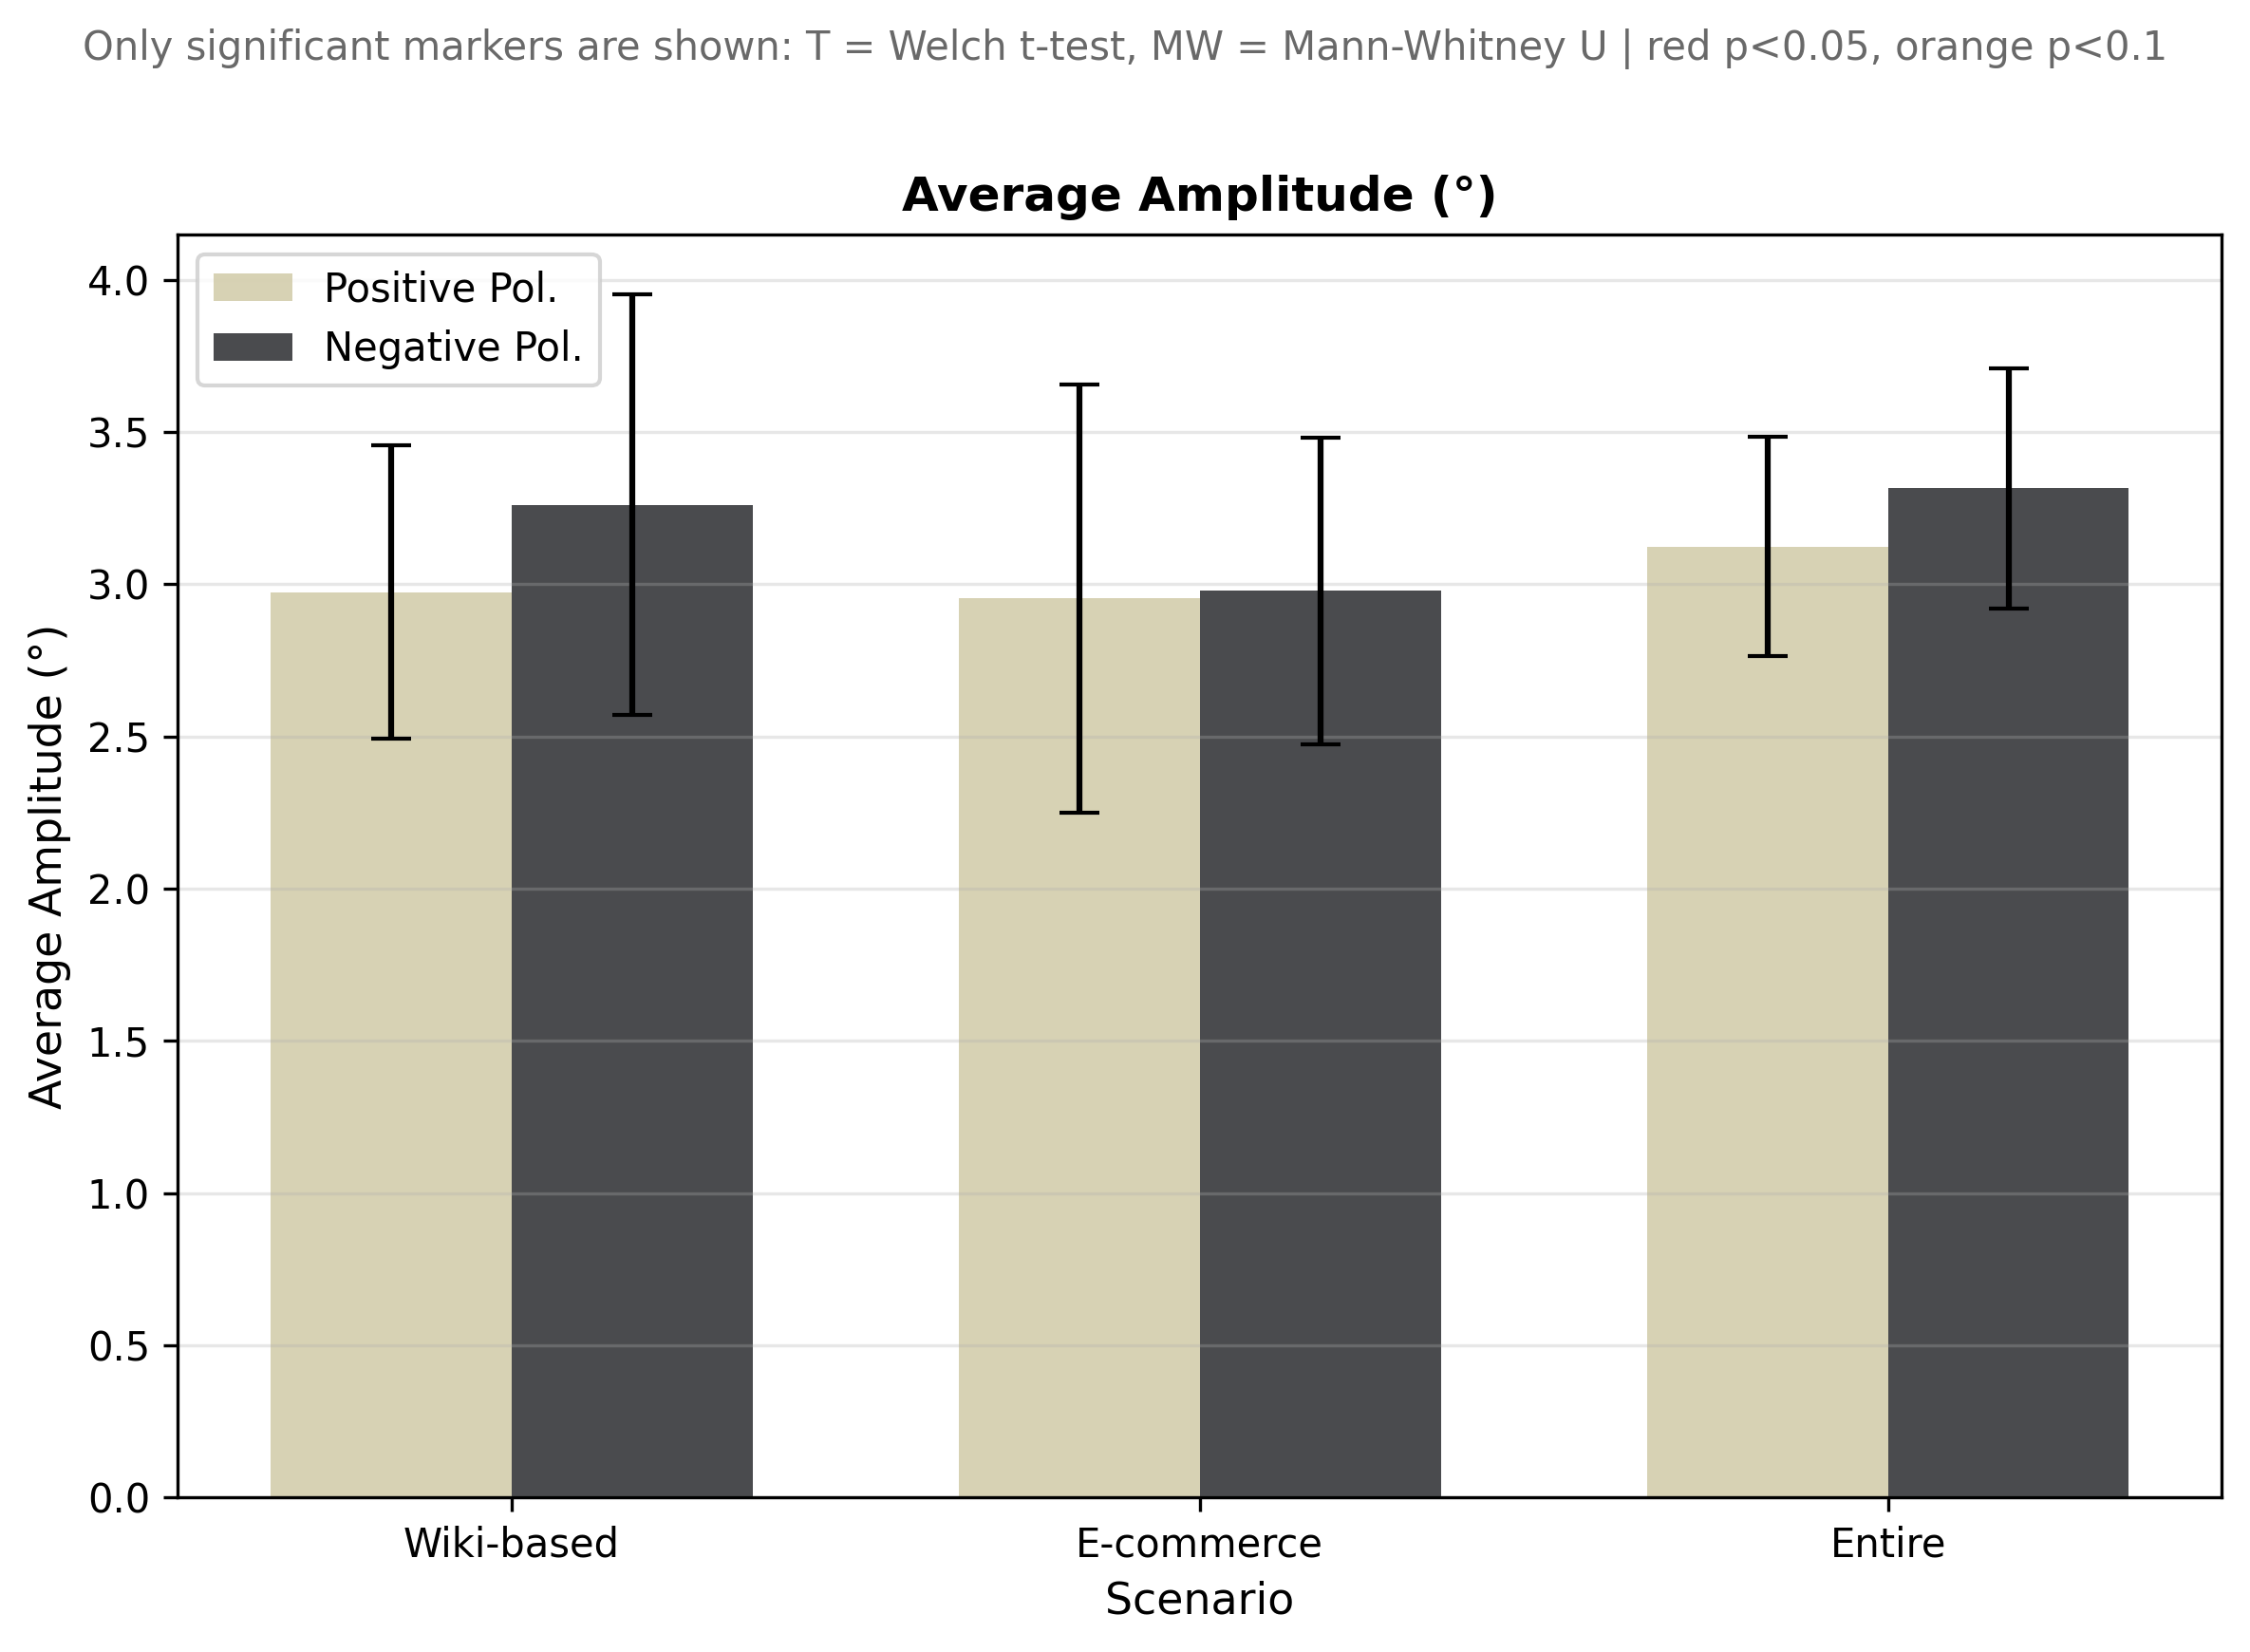
\includegraphics[width=0.8\textwidth]{figures/Average_amplitude_of_saccades.png}
    \caption{Average Saccade Amplitude for each Display Polarity and TOI.}
    \label{fig:asa_boxplot}
\end{figure}
\begin{table}[H]
    \centering
    \small
    \setlength{\tabcolsep}{4pt}
    \caption{Statistics of Average Saccade Amplitude}
    \label{tab:asa_stats}
    \resizebox{0.98\linewidth}{!}{
    \begin{tabular}{|c|c|c|c|c|}
        \hline
        \textbf{TOI} & \textbf{W\textsubscript{PP}} & \textbf{W\textsubscript{NP}} & \textbf{T-Student} & \textbf{Mann-Whitney} \\ \hline
        Wiki-Based & 0.6837 & \textbf{\color{orange}0.0758} & 0.1833 & - \\ \hline
        E-Commerce & \textbf{\color{red}0.0153} & 0.6737 & - & 0.6297 \\ \hline
        Entire Exp. & \textbf{\color{orange}0.0984} & 0.9634 & 0.1620 & - \\ \hline
    \end{tabular}
    }
\end{table}
\subsection{Amplitude of First Saccade}
The amplitude of the first saccade behaved simmilarly to the average saccade amplitude with a pretty even mean distribution.
Followd with a big standard deviation shown in table \ref{tab:afas_basic_stats}. This can be further seen in figure \ref{fig:afas_boxplot} and table \ref{tab:afas_stats}
 this also leads to no significant nor meaningful results in the statistics table \ref{tab:afas_stats}
\begin{table}[H]
    \centering
    \small
    \setlength{\tabcolsep}{4pt}
    \renewcommand{\arraystretch}{1.3}
    \caption{Results of Amplitude of First Saccade}
    \label{tab:afas_basic_stats}

    \resizebox{0.98\linewidth}{!}{
    \begin{tabular}{|c|c|c|c|c|c|}
        \hline
        \textbf{Display Polarity} & \textbf{TOI} & \shortstack{\textbf{Min.} \\ \textbf{(º)}} & \shortstack{\textbf{Mean} \\ \textbf{(º)}} & \shortstack{\textbf{Std.} \\ \textbf{Deviation} \\ \textbf{(º)}} & \shortstack{\textbf{Max.} \\ \textbf{(º)}} \\ \hline
        

        \multirow{3}{*}{Positive Polarity} & \textbf{Wiki-based} & 1.59 & 9.06 & 3.93 & 17.71 \\ \cline{2-6}
         & \textbf{E-Commerce} & 0.56 & 5.35 & 3.29 & 13.00 \\ \cline{2-6}
         & \textbf{Entire Exp.} & 1.07 & 5.18 & 3.97 & 17.74 \\ \hline
        

        \multirow{3}{*}{Negative Polarity} & \textbf{Wiki-based} & 2.03 & 8.74 & 3.79 & 14.09 \\ \cline{2-6}
         & \textbf{E-Commerce} & 0.56 & 4.70 & 3.39 & 14.86 \\ \cline{2-6}
         & \textbf{Entire Exp.} & 0.59 & 6.46 & 4.57 & 17.47 \\ \hline
    \end{tabular}
    }
\end{table}
\begin{figure}[H]
    \centering
    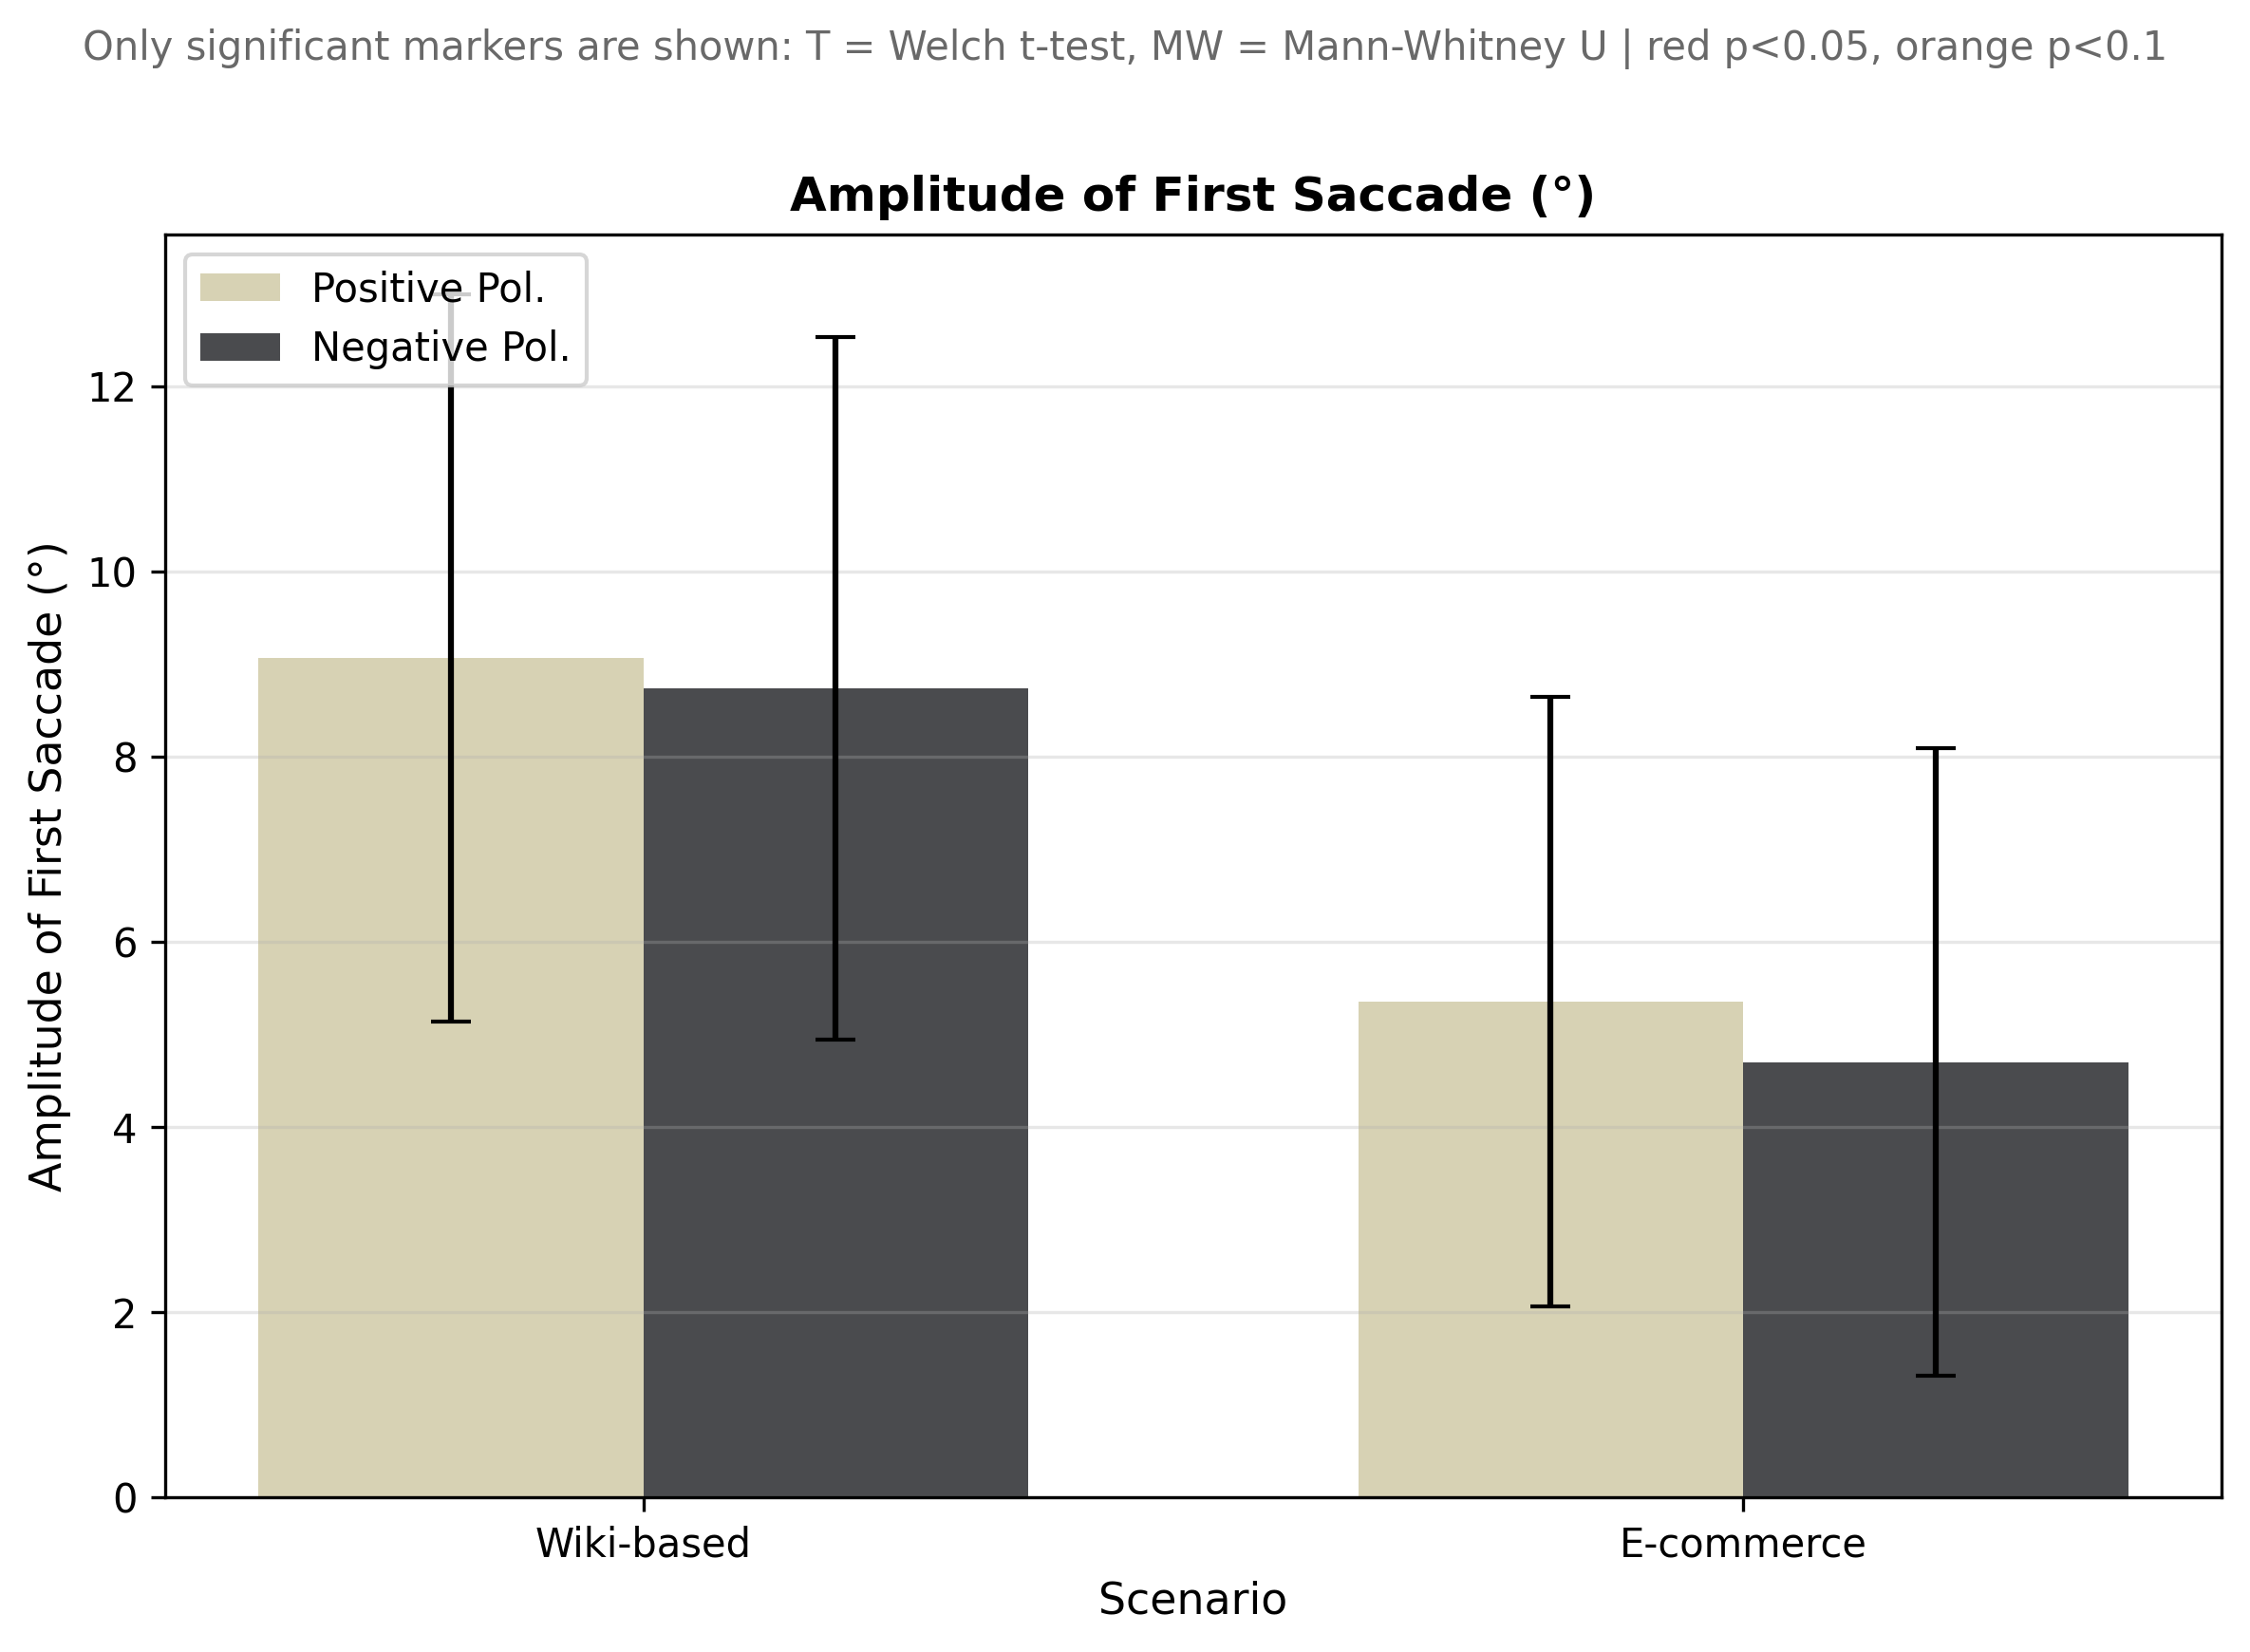
\includegraphics[width=0.8\textwidth]{figures/Amplitude_of_first_saccade.png}
    \caption{Amplitude of First Saccade for each Display Polarity and TOI.}
    \label{fig:afas_boxplot}
\end{figure}
\begin{table}[H]
    \centering
    \small
    \setlength{\tabcolsep}{4pt}
    \caption{Statistics of Amplitude of First Saccade}
    \label{tab:afas_stats}
    \resizebox{0.98\linewidth}{!}{
    \begin{tabular}{|c|c|c|c|c|}
        \hline
        \textbf{TOI} & \textbf{W\textsubscript{PP}} & \textbf{W\textsubscript{NP}} & \textbf{T-Student} & \textbf{Mann-Whitney} \\ \hline
        Wiki-Based & 0.5576 & 0.2155 & 0.8151 & - \\ \hline
        E-Commerce & 0.3231 & \textbf{\color{red}0.0159} & - & 0.5018 \\ \hline
        Entire Exp. & \textbf{\color{red}0.0030} & 0.1831 & - & 0.5353 \\ \hline
    \end{tabular}
    }
\end{table}
\subsection{Number of Saccades}
Lastly, all 3 scenes had a higher mean number of saccades in positive polarity than in negative polarity clearly shown
in table \ref{tab:ns_basic_stats}. 
\begin{table}[H]
    \centering
    \small
    \setlength{\tabcolsep}{4pt}
    \renewcommand{\arraystretch}{1.3}
    \caption{Results of Number of Saccades}
    \label{tab:ns_basic_stats}

    \resizebox{0.98\linewidth}{!}{
    \begin{tabular}{|c|c|c|c|c|c|}
        \hline
        \textbf{Display Polarity} & \textbf{TOI} & \shortstack{\textbf{Min.}} & \shortstack{\textbf{Mean}} & \shortstack{\textbf{Std.} \\ \textbf{Deviation}} & \shortstack{\textbf{Max.}} \\ \hline
        

        \multirow{3}{*}{Positive Polarity} & \textbf{Wiki-based} & 59 & 151.29 & 47.86 & 270 \\ \cline{2-6}
         & \textbf{E-Commerce} & 34 & 184.18 & 83.67 & 305 \\ \cline{2-6}
         & \textbf{Entire Exp.} & 509 & 870.06 & 188.81 & 1122 \\ \hline
        

        \multirow{3}{*}{Negative Polarity} & \textbf{Wiki-based} & 13 & 134.41 & 50.24 & 199 \\ \cline{2-6}
         & \textbf{E-Commerce} & 29 & 171.47 & 59.10 & 241 \\ \cline{2-6}
         & \textbf{Entire Exp.} & 344 & 746.41 & 166.22 & 1004 \\ \hline
    \end{tabular}
    }
\end{table}
There's only a relevant results regardin the whole recording with a p-value of 0.0582 in the t-student test. It is not enough to be 
considered relevant but gets close enough to be considered relevant. This can be further seen in figure \ref{fig:ns_boxplot} and table \ref{tab:ns_stats}.
\begin{figure}[H]
    \centering
    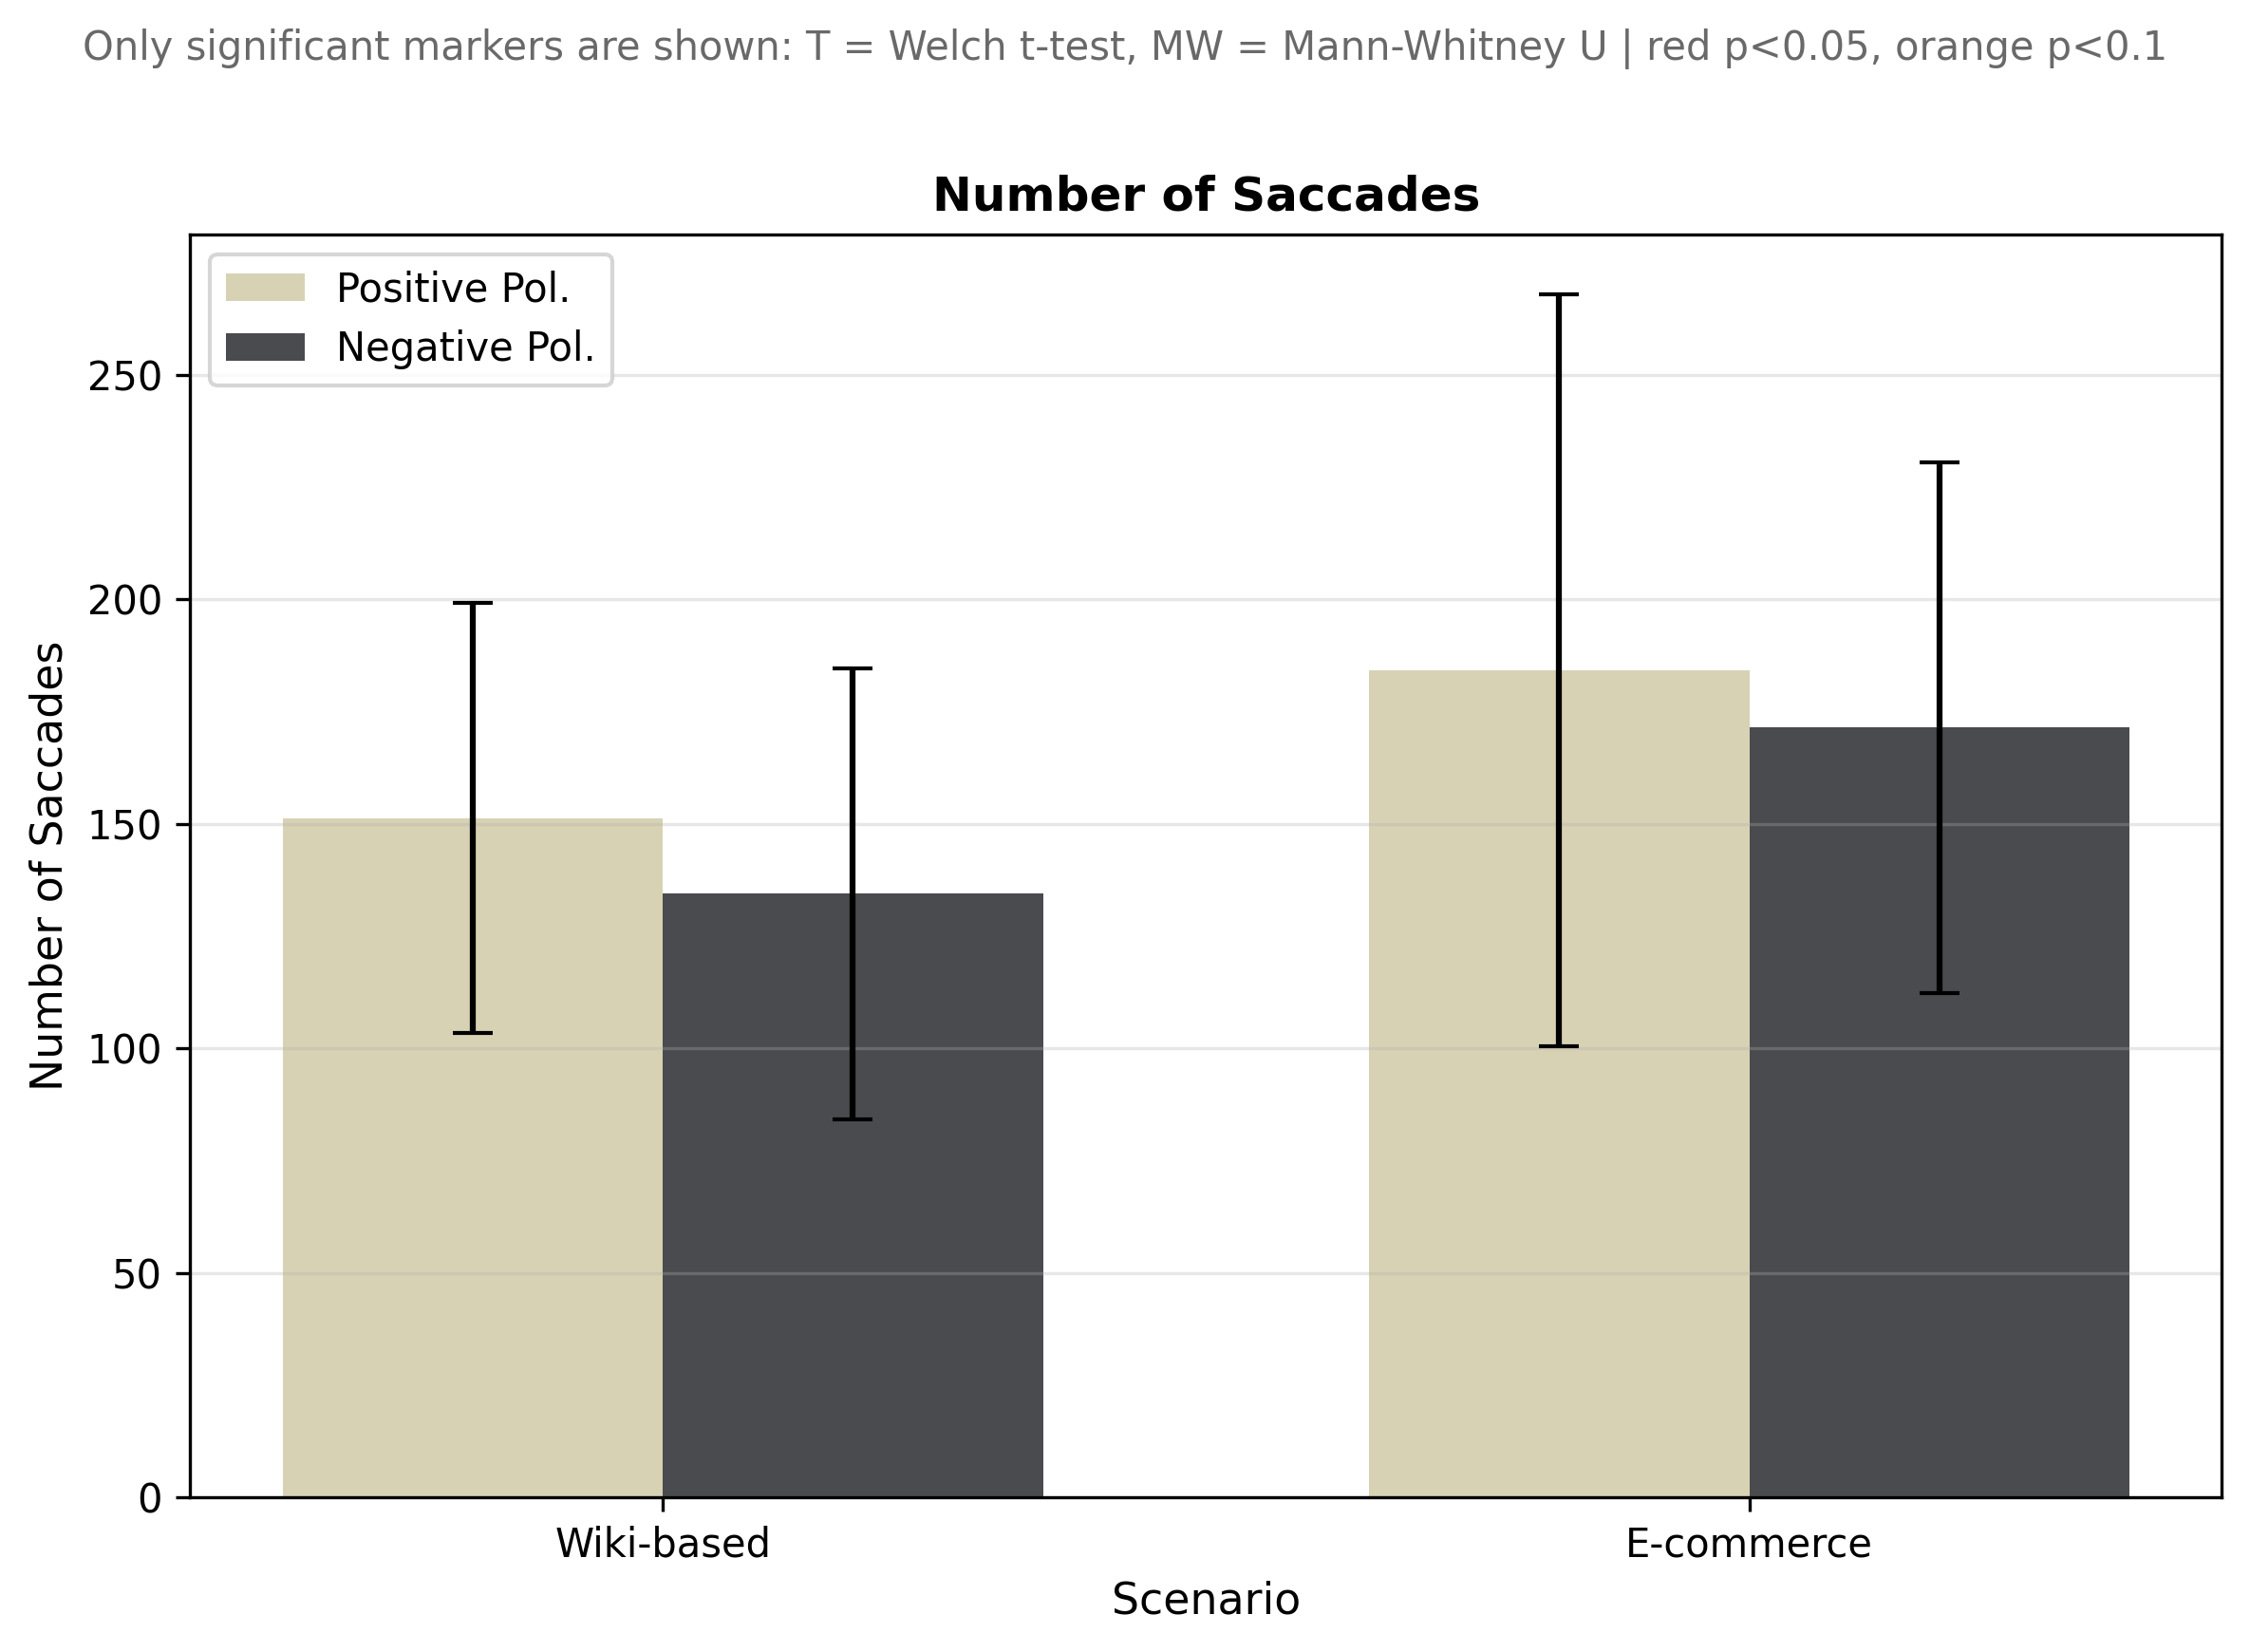
\includegraphics[width=0.8\textwidth]{figures/Number_of_saccades.png}
    \caption{Number of Saccades for each Display Polarity and TOI.}
    \label{fig:ns_boxplot}
\end{figure}
\begin{table}[H]
    \centering
    \small
    \setlength{\tabcolsep}{4pt}
    \caption{Statistics of Number of Saccades}
    \label{tab:ns_stats}
    \resizebox{0.98\linewidth}{!}{
    \begin{tabular}{|c|c|c|c|c|}
        \hline
        \textbf{TOI} & \textbf{W\textsubscript{PP}} & \textbf{W\textsubscript{NP}} & \textbf{T-Student} & \textbf{Mann-Whitney} \\ \hline
        Wiki-Based & 0.9486 & 0.2609 & 0.3377 & - \\ \hline
        E-Commerce & 0.1768 & \textbf{\color{red}0.0185} & - & 0.3797 \\ \hline
        Entire Exp. & 0.1577 & 0.6058 & \textbf{\color{orange}0.0582} & - \\ \hline
    \end{tabular}
    }
\end{table}
\section{Questionnaire Results}
This section will provide an insight of the results obtained through the Google Forms
Questionnaire. The results will be shown along with an ID, this ID corresponds to
the first letter of the subsection name in the section \ref{sec:final_questionnaire} 
followed by the number of the question. For example, the first question of the Wiki-Based
Scene will be identified as W1, the second question of the E-Commerce Scene will be identified 
as E2 and so on.
\subsection{Reading Comprehension Questions}
\subsubsection{Wiki-Based}
Overall results seen in table \ref{tab:rcq_wiki_results} show that the percentage of correct answers 
is higher in negative polarity than in positive polarity in every question but in $W3$ where
the differences are pretty steep.
\begin{table}[H]
    \centering
    \small
    \setlength{\tabcolsep}{4pt}
    \renewcommand{\arraystretch}{1.3}
    \caption{Basic data per question of the Wiki-Based Scene}
    \label{tab:rcq_wiki_results}

    \resizebox{0.98\linewidth}{!}{
    \begin{tabular}{|c|c|c|c|c|}
        \hline
        \textbf{Question ID} & \textbf{Correct Answers} & \textbf{Wrong Answers} & \textbf{PP Correct(\%)} & \textbf{NP Correct(\%)} \\ \hline
        W1 & 15 & 19 & 29.41 & 58.82 \\ \hline
        W2 &  21 & 13 & 41.18 & 82.36\\ \hline
        W3 &  20 & 14 & 70.59 & 47.06\\ \hline
        W4 &  24 & 10 & 64.71 & 76.47 \\ \hline
    \end{tabular}
    }
\end{table}
\subsubsection{E-Commerce}
E-Commerce results in table \ref{tab:rcq_ecommerce_results} show a pretty even distribution of 
correct answers between both polarities. The question $E3$ is surprisingly a bit lower in 
negative polarity as this question was pretty simple.
\begin{table}[H]
    \centering
    \small
    \setlength{\tabcolsep}{4pt}
    \renewcommand{\arraystretch}{1.3}
    \caption{Basic data per question of the E-Commerce Scene}
    \label{tab:rcq_ecommerce_results}

    \resizebox{0.98\linewidth}{!}{
    \begin{tabular}{|c|c|c|c|c|}
        \hline
        \textbf{Question ID} & \textbf{Correct Answers} & \textbf{Wrong Answers} & \textbf{PP Correct(\%)} & \textbf{NP Correct(\%)} \\ \hline
        E1 & 34 & 0 & 100 & 100 \\ \hline
        E2 &  18 & 16 & 47.06 & 58.83 \\ \hline
        E3 &  28 & 6 & 88.24 & 76.47\\ \hline
        E4 &  21 & 13 & 64.71 & 58.82 \\ \hline
    \end{tabular}
    }
\end{table}
\subsection{Preference Questions}
The questionnaire is divided in two types of questions, categorical and numeric. The categorial questions are those
where the participant chooses from a non numeric list of options. For example, In question P1 the participant had to choose
between "Normal Vision" and "Corrected Vision". On the other hand, the numeric questions are those where 
the experimentee answers with a numerical value.
\subsubsection{Categorical Questions}
The experiment remained consistent not only in gender and age distribution as seen in chapter \ref{chap:methodology}
but also in the type of vision of the participants as shown in table \ref{tab:participants_vision}. This consistency 
results in a 53\% of participants with normal vision and a 47\% of participants with corrected vision in both polarities.
\begin{table}[H]
    \centering
    \caption{Type of vision of the participants (Question P1)}
    \label{tab:participants_vision}
    \begin{tabular}{|c|c|c|}
        \hline
        \textbf{Polarity} & \textbf{Normal Vision} & \textbf{Corrected Vision} \\ \hline
        Positive Polarity & 9 & 8 \\ \hline
        Negative Polarity & 9 & 8 \\ \hline
    \end{tabular}
\end{table}
The display polarity preference for both scenes shows a slight preference for white background with black text 
in the Wiki-Based scene as shown in table \ref{tab:wiki_preference}
\begin{table}[H]
    \centering
    \caption{Wiki-Based Scene Preference (Question P2)}
    \label{tab:wiki_preference}
    \begin{tabular}{|c|c|c|}
        \hline
        \textbf{Experiment Polarity} & \textbf{\shortstack{Positive Polarity\\Preferred}} & \textbf{\shortstack{Negative Polarity\\Preferred}} \\ \hline
        Positive Polarity & 11 & 6 \\ \hline
        Negative Polarity & 9 & 8 \\ \hline
    \end{tabular}
\end{table}
The trend in the E-Commerce scene is simmilar to the Wiki-Based scene having an increase for 
the positive polarity as seen in table \ref{tab:ecommerce_preference}.
\begin{table}[H]
    \centering
    \caption{E-Commerce Scene Preference (Question P3)}
    \label{tab:ecommerce_preference}
    \begin{tabular}{|c|c|c|}
        \hline
        \textbf{Experiment Polarity} & \textbf{\shortstack{Positive Polarity\\Preferred}} & \textbf{\shortstack{Negative Polarity\\Preferred}} \\ \hline
        Positive Polarity & 11 & 6 \\ \hline
        Negative Polarity & 12 & 5 \\ \hline
    \end{tabular}
\end{table}
\subsubsection{Numeric Questions}
Regardin the numeric questions, the results in table \ref{tab:numeric_descriptor} should be read along with the 
questions in chapter \ref{sec:final_questionnaire} to understand every question. Overall, the results appeared 
to be pretty even between polarities.
\begin{table}[H]
    \centering
    \small
    \setlength{\tabcolsep}{4pt}
    \renewcommand{\arraystretch}{1.3}
    \caption{Numeric Preference Descriptive Statistics}
    \label{tab:numeric_descriptor}

    \resizebox{0.98\linewidth}{!}{
    \begin{tabular}{|c|c|c|c|c|c|}
        \hline
        \textbf{Question ID} & \textbf{Display Polarity} & \textbf{Min.} & \textbf{Mean} & \textbf{Std. Deviation} & \textbf{Max.} \\ \hline
           \multirow{2}{*}{P4} & Positive & 1 & 3.29 & 1.36 & 5 \\ \cline{2-6}
            & Negative & 1 & 3.65 & 1.41 & 5 \\ \hline
           \multirow{2}{*}{P5} & Positive & 1 & 2.82 & 1.51 & 5 \\ \cline{2-6}
            & Negative & 1 & 2.76 & 1.48 & 5 \\ \hline
           \multirow{2}{*}{P6} & Positive & 3 & 4.00 & 0.71 & 5 \\ \cline{2-6}
            & Negative & 2 & 4.24 & 0.90 & 5 \\ \hline
           \multirow{2}{*}{P7} & Positive & 2 & 3.71 & 0.85 & 5 \\ \cline{2-6}
            & Negative & 2 & 3.65 & 0.79 & 5 \\ \hline
           \multirow{2}{*}{P8} & Positive & 2 & 3.76 & 0.75 & 5 \\ \cline{2-6}
            & Negative & 2 & 3.88 & 0.93 & 5 \\ \hline
           \multirow{2}{*}{P9} & Positive & 3 & 4.00 & 0.87 & 5 \\ \cline{2-6}
            & Negative & 2 & 3.59 & 0.87 & 5 \\ \hline
           \multirow{2}{*}{P10} & Positive & 2 & 3.47 & 0.94 & 5 \\ \cline{2-6}
            & Negative & 2 & 3.47 & 1.07 & 5 \\ \hline
           \multirow{2}{*}{P11} & Positive & 1 & 3.41 & 1.37 & 5 \\ \cline{2-6}
            & Negative & 1 & 3.35 & 1.00 & 5 \\ \hline
           \multirow{2}{*}{P12} & Positive & 3 & 4.12 & 0.78 & 5 \\ \cline{2-6}
            & Negative & 3 & 4.41 & 0.71 & 5 \\ \hline
    \end{tabular}
    }
\end{table}
In adition, the statistical tests in table \ref{tab:numeric_statistics} show no significant results 
with all p-values being pretty far from the significance level. It is also important to note how none 
of the questions followed a normal distribution, this is probably related to the likert scale used in the questionnaire.
\begin{table}[H]
    \centering
    \small
    \setlength{\tabcolsep}{4pt}
    \renewcommand{\arraystretch}{1.3}
    \caption{Numeric Preference Statistical Tests}
    \label{tab:numeric_statistics}

    \resizebox{0.98\linewidth}{!}{
    \begin{tabular}{|c|c|c|c|c|}
        \hline
        \textbf{Question ID} & \textbf{W\textsubscript{PP}} & \textbf{W\textsubscript{NP}} & \textbf{T-Student} & \textbf{Mann-Whitney} \\ \hline
        P4 & \textbf{\color{red}0.014450} & \textbf{\color{red}0.008111} & - & 0.443897 \\ \hline
        P5 & \textbf{\color{red}0.018117} & \textbf{\color{red}0.027799} & - & 0.943579 \\ \hline
        P6 & \textbf{\color{red}0.003247} & \textbf{\color{red}0.001766} & - & 0.266670 \\ \hline
        P7 & \textbf{\color{red}0.033180} & \textbf{\color{red}0.022905} & - & 0.867835 \\ \hline
        P8 & \textbf{\color{red}0.006383} & \textbf{\color{red}0.024222} & - & 0.698056 \\ \hline
        P9 & \textbf{\color{red}0.001513} & \textbf{\color{red}0.029538} & - & 0.230296 \\ \hline
        P10 & \textbf{\color{red}0.039537} & \textbf{\color{red}0.017035} & - & 0.928482 \\ \hline
        P11 & \textbf{\color{red}0.047147} & \textbf{\color{red}0.045448} & - & 0.815614 \\ \hline
        P12 & \textbf{\color{red}0.003016} & \textbf{\color{red}0.000501} & - & 0.263356 \\ \hline

    \end{tabular}
    }
\end{table}
\chapter{Discussion}
\label{chap:discussion}
\section{Wiki-Based}
The wiki-based part of the experiment has shown none relevant or significant results. However, 
this points that for the hypothesis stated before, the reading of texts may be equally treated 
in both polarities in a wiki-based webpage. These results can lead to theories, either
the reading task was not long enough to induce difficulties or daily users are highly adapted to
both polarities due to the wide use of the internet. 


\begin{figure}[H]
    \centering
    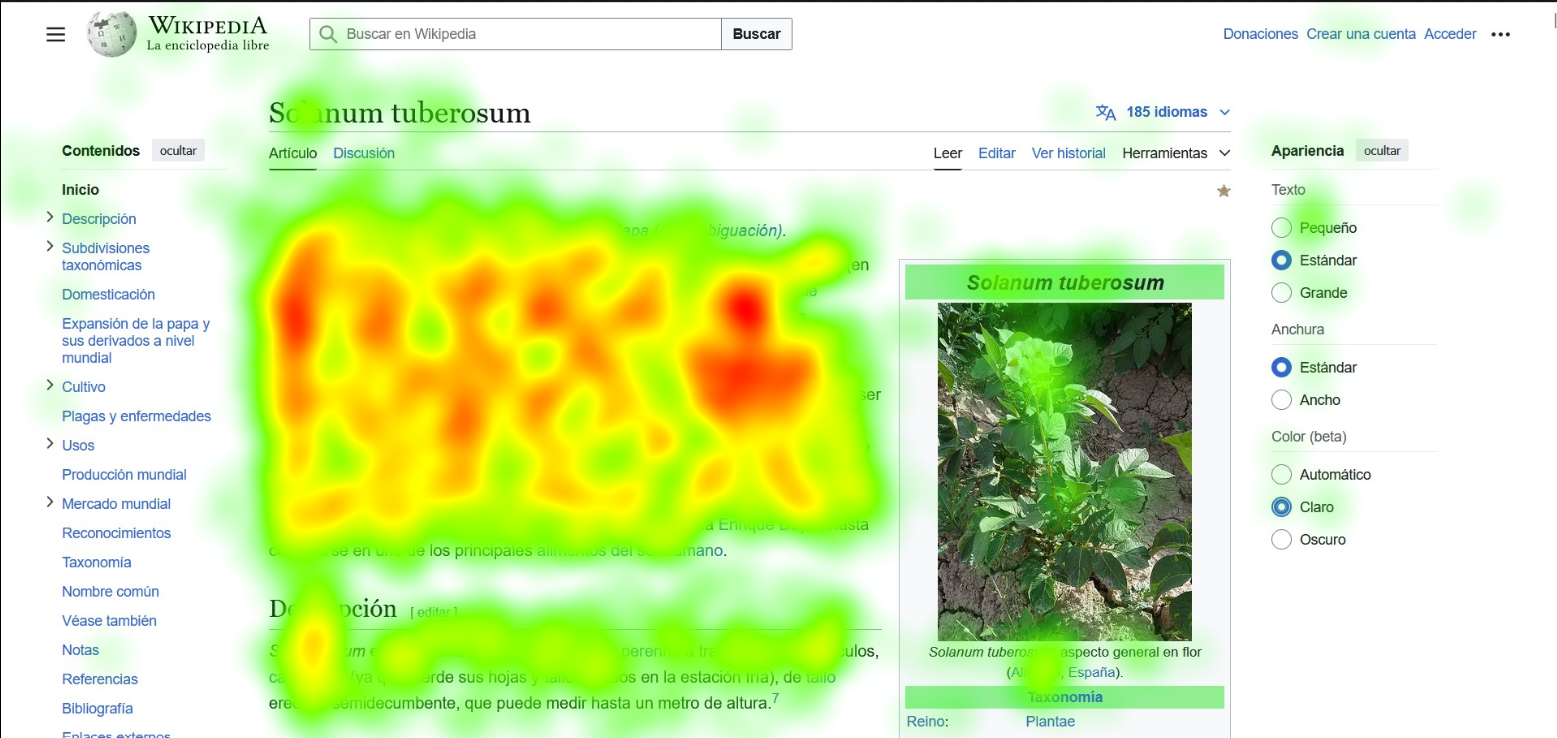
\includegraphics[width=0.85\textwidth]{figures/PaataFix.png}
    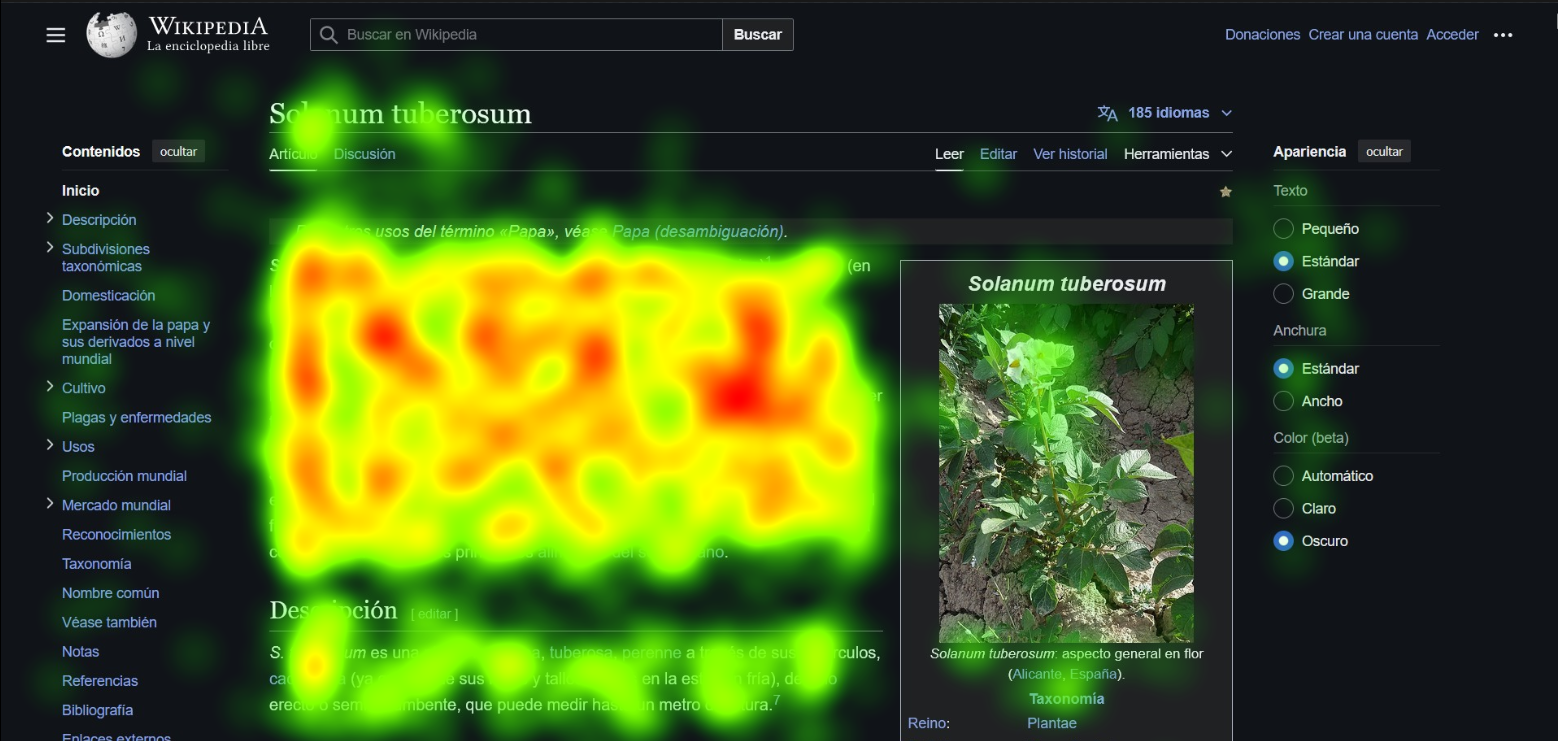
\includegraphics[width=0.85\textwidth]{figures/PatataOscFix.png}
    \caption{Fixations heatmap of wiki-based experiment. First image 
    positive polarity, second image negative polarity.}
    \label{fig:wiki-results}
\end{figure}

Regarding the preference of users in this scenario, overall users prefer positive polarity over negative polarity 
supporting the hypothesis H3.
However, when the users of negative polarity were asked the preference, the results were evenly distributed 
between both polarities and the comprehension questions had an even distribution of correct percentages.
\section{E-Commerce}
The e-commerce part has no significant results either, however there is a variable that was 
relevant and almost significant, the average duration of fixations. As expressed in the chapter \ref{chap:data_analysis}
this variable is related to the difficulty of reading this can be an indicator for the hypothesiis H1 analyzing the result
of this variable. There's proof that users may have less difficulty reading in the negative polarity
than in the positive polarity. Although as the result is not significant but relevant, more research is needed 
to confirm this hypothesis.
\begin{figure}[H]
    \centering
    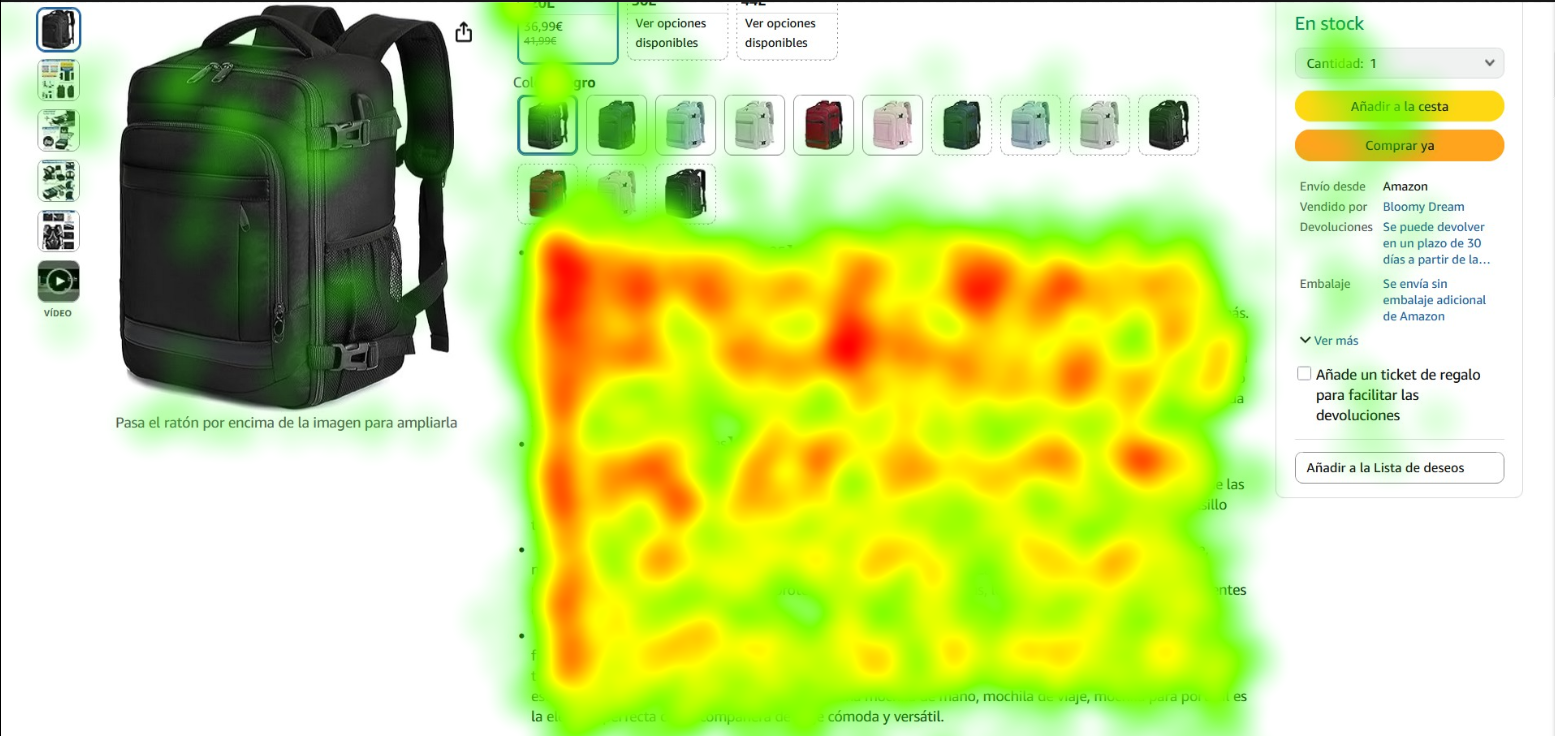
\includegraphics[width=0.8\textwidth]{figures/MochilaClarFix.png}
    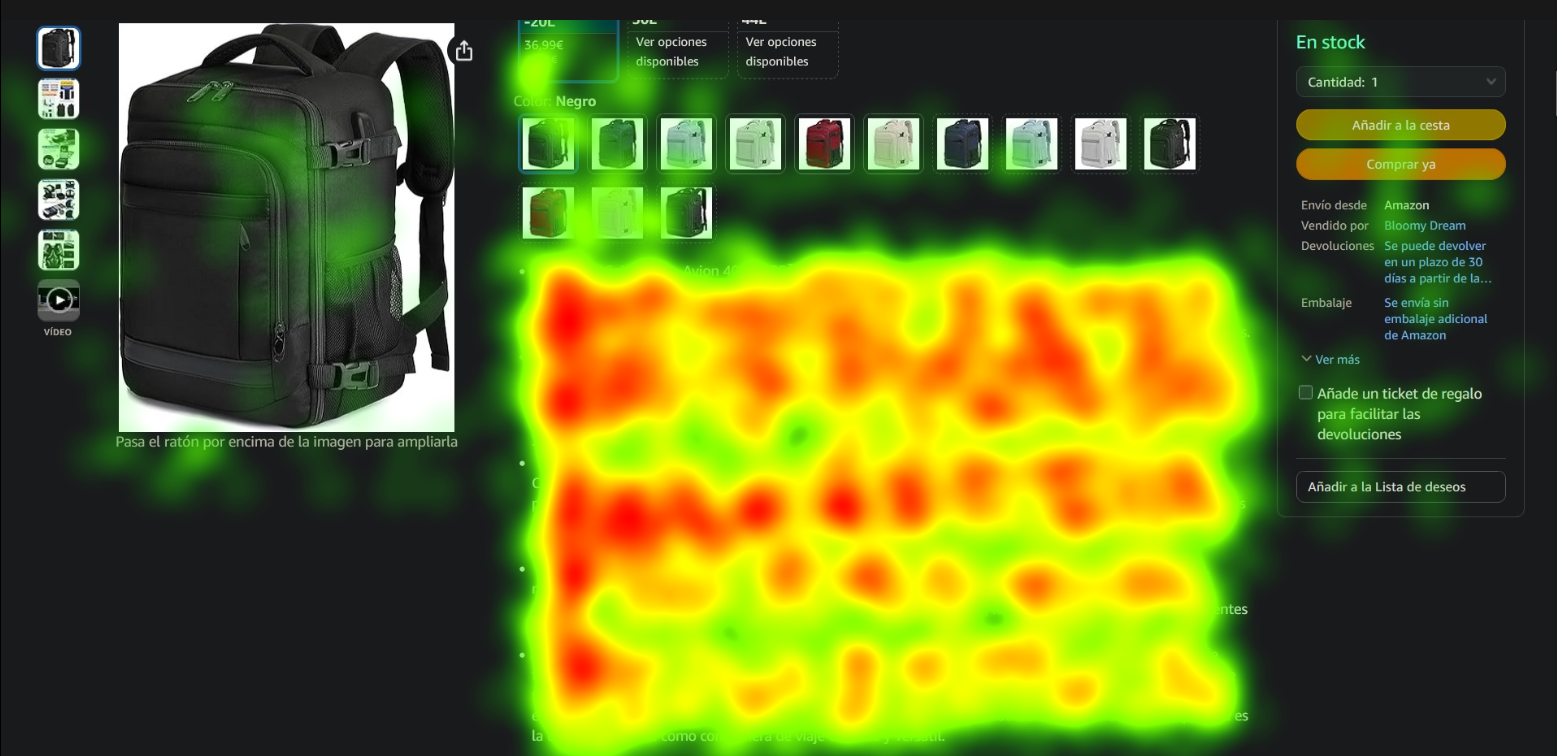
\includegraphics[width=0.8\textwidth]{figures/MochilaOscFix.png}
    \caption{Fixations heatmap of e-commerce experiment. First image 
    positive polarity, second image negative polarity.}
    \label{fig:moch-results}
\end{figure}

The reading questions had a high pecentage of correct answers in both polarities, in addition, the
preference of users was higher overall for the positive polarity with a higher difference than the wiki-based scenario.
Supporting the hypothesis H3 of users prefering positive polarity over negative polarity.
\section{Preference Questionnaires}
None of the questions regarding preference had significant results. However, the results
indicate that users used more the positive polarity daily than the negative polarity. 
Both of them shared the same percentage of users finding the webpages professional and 
appealing. Both groups agreed that the colors used in their experiment made the text
easier to read. 



\chapter{Conclusion}
\label{chap:conclusion_and_future_work}
The trend since the early 2000s has been to move towards negative polarity, there was no explanation
whether the trend was due to efficiency or design factors. This thesis aimed on clarifying the reasons 
on why this was happening. After investigating 34 different subjects in common scenarios such as wiki-based
 and e-commerce the data revealed no significant difference between the two polarities. Therefore the conclusion 
 of this thesis is that there are not enough evidence to support the advantages of positive polarity over negative polarity.
However it is worth mentioning that users do prefer positive polarity over negative polarity, accepting the hypothesis H3 of this project.

\section{Future Work}
The future work of this project shoudl be focused in the following ideas:
\begin{itemize}
    \item \textbf{Sample Size:} The sample size of this project is short, increasing the sample may reveal significant results.
    \item \textbf{Precise Regression Study:} The regressions were calculated with a rough calculation, there may be tools
    that provide this variable with more precision.
    \item \textbf{Longer Exposure:} The experiment is centered around texts however, the expsure and time spent reading may reveal new 
    results by expanding the time of the experiment.
    \item \textbf{Sample Age:} The sample of the project is focused on young people, they have been adapted and exposed to new technologies
    since they were born, providing a older sample may reveal new results as older people have not adapted entirely to the internet and its design.
\end{itemize}

\printbibliography % Imprime la lista de referencias al final

\appendix
\cleardoublepage

\chapter{Project Management}
\label{app:project_management}
\section{Planning}
\subsection{Stakeholders}
This project can be appealing to a wide variety of Stakeholders. Firstly, the academic community
can be interested in the results to provide a new perspective of the influence of colors in users. 
It can also benefit the bursting internet industry where the user experience has become a key factor.
Given this knowledge, the project can be interesting for:
\begin{itemize}
    \item Psichology Researchers
    \item Human-Computer Interaction Researchers
    \item General Users
    \item Software Community and Students
    \item Private Companies that have a frontend product.
    \item Public Institutions 
\end{itemize}
\subsection{Organization Breakdown Structure (OBS) and Product Breakdown Structure (PBS)}
The OBS of the project as seen in figure \ref{fig:OBS} follows a hierarchical structure with three levels. 
Being the Project Manager the leader of this project and the one in charge of coordinating the software
engineer and the Lead Researcher. Secondly, the Lead Researcher is in charge of both junior researchers who
should be persons with knowledge in the field of computing and human computer interaction.
\begin{figure}[H]
    \centering
    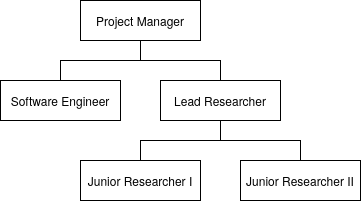
\includegraphics[width=0.7\textwidth]{figures/OBS.png}
    \caption{Organization Breakdown Structure (OBS)}
    \label{fig:OBS}
\end{figure}
There exists two main products which compose the Product Breakdown Structure (PBS) whcih then each of them have
different subtasks to develop them.
\begin{enumerate}
    \item \textbf{Experiment:} This is the main product where all the work is focused on. It is composed of three subtasks:
    \begin{enumerate}
        \item \textbf{Experiment Proposal:} The State of the Art and previous planning of the experiment.
        \item \textbf{Experiment Development:} The execution of the planned experiment.
        \item \textbf{Data Analysis:} The processing and analysis of the obtained data.
    \end{enumerate}
    \item \textbf{Documentation:} The final objective is to document the whole process into a scientific paper.
\end{enumerate}

The PBS described have a relation to the OBS as seen in table \ref{tab:rel_OBS_PBS}.
\begin{table}[H]
    \centering
    \caption{Relation between OBS and PBS}
    \label{tab:rel_OBS_PBS}
    \begin{tabularx}{\textwidth}{|>{\raggedright\arraybackslash}X|>{\raggedright\arraybackslash}X|>{\raggedright\arraybackslash}X|}
        \hline
        \textbf{Task} & \textbf{Resource} & \textbf{Product} \\
        \hline
        \textbf{State of the Art} & Junior Researchers, Lead Researcher & Experiment Proposal \\
        \hline
        \textbf{Previous Planning} & Project Manager, Lead Researcher & Experiment Proposal \\
        \hline
        \textbf{Experiment Planning} & Software Engineer, Lead Researcher & Experiment Development \\
        \hline
        \textbf{Experiment Execution} & Junior Researchers & Experiment Development \\
        \hline
        \textbf{Tobii Preparations} & Software Engineer & Experiment Development \\
        \hline
        \textbf{Data Preprocessing} & Software Engineer, Junior Researchers & Data Analysis \\
        \hline
        \textbf{Data Processing} & Software Engineer & Data Analysis \\
        \hline
        \textbf{Statistical Study} & Lead Resercher & Data Analysis \\
        \hline
        \textbf{Paper Writing} & Junior Researchers & Documentation \\
        \hline
        \textbf{Paper Review} & Lead Researcher  & Documentation \\
        \hline
    \end{tabularx}
\end{table}
\section{Risk Identification and Management}
Risk identification is a key phase of the project as it can help acknowledge possible negative 
effects on the project. It is important to have a strategy to face such events in order to make 
them affect the least possible the outcome of the project.
\begin{table} [H]
    \centering
    \caption{Risks List}
    \label{tab:risks}
    \begin{tabularx}{0.8\textwidth} { 
        | >{\raggedright\arraybackslash}c 
        | >{\centering\arraybackslash}X| }
        \hline \textbf{Risk ID} & \textbf{Risk Name} \\
        \hline
        \textbf{1} & Few Experimental Samples \\
        \hline
        \textbf{2} & Statistical Analysis Imprecision \\
        \hline
        \textbf{3} & Loss of Partial Work \\
        \hline
        \textbf{4} & Justified Leave of Worker \\
        \hline
        \textbf{5} & Lack of Teamwork \\
        \hline
        \textbf{6} & Tobii Measurements Drifts \\
        \hline
        \textbf{7} & Privacy Violations \\
        \hline
        \textbf{8} & Timeline Delay \\
        \hline
        \textbf{9} & Publisher Rejection \\
        \hline
    \end{tabularx}
\end{table}
\subsection{Risk Details}
\label{sub:risk_details}
\subsubsection{Few Experimental Samples}
There is not enough sample for the test, this can lead to inconsistent
 data and problems when doing the processing and publishing the paper.
\begin{table}[H]
    \centering
    \small
    \renewcommand{\arraystretch}{1.8}
    \setlength{\tabcolsep}{3pt} 
    
    \caption{Few experimental samples impact.}
    \label{tab:risk_impact}
    
    \begin{tabularx}{\textwidth}
        {|>{\centering\arraybackslash}X|>{\centering\arraybackslash}X|>{\centering\arraybackslash}X|>
        {\centering\arraybackslash}X|>{\centering\arraybackslash}X|>{\centering\arraybackslash}p{1.5cm}|}
        \hline
        \multirow{2}{*}{\textbf{Probability}} & \multicolumn{4}{c|}{\textbf{Impact}} 
        & \multirow{2}{*}{\textbf{Impact}} \\ \cline{2-5}
        
        & \textbf{Budget} & \textbf{Planning} & \textbf{Reach} & \textbf{Quality} & \\ \hline
        
        Medium & Low & Low & Medium & Critic & \cellcolor{orange} 0,45 \\ \hline
    \end{tabularx}
\end{table}
\subsubsection{Statistical Analysis Imprecision}
When analyzing the processed data if the statistic analysis is imprecise it can lead to wrong 
conclusions. It is important for it to remain precise.
\begin{table} [H]
    \centering
    \small
    \renewcommand{\arraystretch}{1.8}
    \setlength{\tabcolsep}{3pt} 
    
    \caption{Statistical analysis imprecision impact.}
    \label{tab:risk_impact2}
    
    \begin{tabularx}{\textwidth}
        {|>{\centering\arraybackslash}X|>{\centering\arraybackslash}X|>{\centering\arraybackslash}X|>
        {\centering\arraybackslash}X|>{\centering\arraybackslash}X|>{\centering\arraybackslash}p{1.5cm}|}
        \hline
        \multirow{2}{*}{\textbf{Probability}} & \multicolumn{4}{c|}{\textbf{Impact}} 
        & \multirow{2}{*}{\textbf{Impact}} \\ \cline{2-5}
        
        & \textbf{Budget} & \textbf{Planning} & \textbf{Reach} & \textbf{Quality} & \\ \hline
        
        Low & Seamless & Low & Low & Medium & \cellcolor{green!40} 0,09 \\ \hline
    \end{tabularx}
\end{table}
\subsubsection{Loss of Partial Work}
Due to data corruption or any other external agent, there’s a possibility of losing the entire 
or part of the work accomplished.
\begin{table}[H]
    \centering
    \small
    \renewcommand{\arraystretch}{1.8}
    \setlength{\tabcolsep}{3pt} 
    
    \caption{Loss of partial work impact.}
    \label{tab:risk_impact3}
    
    \begin{tabularx}{\textwidth}
        {|>{\centering\arraybackslash}X|>{\centering\arraybackslash}X|>{\centering\arraybackslash}X|>
        {\centering\arraybackslash}X|>{\centering\arraybackslash}X|>{\centering\arraybackslash}p{1.5cm}|}
        \hline
        \multirow{2}{*}{\textbf{Probability}} & \multicolumn{4}{c|}{\textbf{Impact}} 
        & \multirow{2}{*}{\textbf{Impact}} \\ \cline{2-5}
        
        & \textbf{Budget} & \textbf{Planning} & \textbf{Reach} & \textbf{Quality} & \\ \hline
        
        Low & Medium & High & Medium & Low & \cellcolor{green!40} 0,17 \\ \hline
    \end{tabularx}
\end{table}
\subsubsection{Justified Leave of Worker}
Any of the workers may need a justified leave of work according to the Spanish law.
\begin{table}[H]
    \centering
    \small
    \renewcommand{\arraystretch}{1.8}
    \setlength{\tabcolsep}{3pt} 
    
    \caption{Justified leave of worker impact.}
    \label{tab:risk_impact4}
    
    \begin{tabularx}{\textwidth}
        {|>{\centering\arraybackslash}X|>{\centering\arraybackslash}X|>{\centering\arraybackslash}X|>
        {\centering\arraybackslash}X|>{\centering\arraybackslash}X|>{\centering\arraybackslash}p{1.5cm}|}
        \hline
        \multirow{2}{*}{\textbf{Probability}} & \multicolumn{4}{c|}{\textbf{Impact}} 
        & \multirow{2}{*}{\textbf{Impact}} \\ \cline{2-5}
        
        & \textbf{Budget} & \textbf{Planning} & \textbf{Reach} & \textbf{Quality} & \\ \hline
        
        Medium & Low & High & Low & Low & \cellcolor{yellow} 0,28 \\ \hline
    \end{tabularx}
\end{table}
\subsubsection{Lack of Teamwork}
Teamwork is important as it creates a healthy environment where workers feel comfortable, 
however it is quite easy to have a lot of individualism in teams.
\begin{table} [H]
    \centering
    \small
    \renewcommand{\arraystretch}{1.8}
    \setlength{\tabcolsep}{3pt} 
    
    \caption{Lack of teamwork impact.}
    \label{tab:risk_impact5}
    
    \begin{tabularx}{\textwidth}
        {|>{\centering\arraybackslash}X|>{\centering\arraybackslash}X|>{\centering\arraybackslash}X|>
        {\centering\arraybackslash}X|>{\centering\arraybackslash}X|>{\centering\arraybackslash}p{1.5cm}|}
        \hline
        \multirow{2}{*}{\textbf{Probability}} & \multicolumn{4}{c|}{\textbf{Impact}} 
        & \multirow{2}{*}{\textbf{Impact}} \\ \cline{2-5}
        
        & \textbf{Budget} & \textbf{Planning} & \textbf{Reach} & \textbf{Quality} & \\ \hline
        
        Medium & Low & High & Low & Low & \cellcolor{green!40} 0,15 \\ \hline
    \end{tabularx}
\end{table}
\subsubsection{Tobii Measurements Drifts}
Due to light changes, the subject of the experiment looking away or other uncontrollable 
events, the tobii eye-tracker may drift its measurements.
\begin{table} [H]
    \centering
    \small
    \renewcommand{\arraystretch}{1.8}
    \setlength{\tabcolsep}{3pt} 
    
    \caption{Tobii measurements drifts impact.}
    \label{tab:risk_impact6}
    
    \begin{tabularx}{\textwidth}
        {|>{\centering\arraybackslash}X|>{\centering\arraybackslash}X|>{\centering\arraybackslash}X|>
        {\centering\arraybackslash}X|>{\centering\arraybackslash}X|>{\centering\arraybackslash}p{1.5cm}|}
        \hline
        \multirow{2}{*}{\textbf{Probability}} & \multicolumn{4}{c|}{\textbf{Impact}} 
        & \multirow{2}{*}{\textbf{Impact}} \\ \cline{2-5}
        
        & \textbf{Budget} & \textbf{Planning} & \textbf{Reach} & \textbf{Quality} & \\ \hline
        
        High & Seamless & Seamless & Seamless & Medium & \cellcolor{yellow} 0,21 \\ \hline
    \end{tabularx}
\end{table}
\subsubsection{Privacy Violations}
This whole research gathers a lot of sensitive information and it is a key to store and 
manipulate the sensitive data correctly as it can lead to fines.
\begin{table} [H]
    \centering
    \small
    \renewcommand{\arraystretch}{1.8}
    \setlength{\tabcolsep}{3pt} 
    
    \caption{Privacy violations impact.}
    \label{tab:risk_impact7}
    
    \begin{tabularx}{\textwidth}
        {|>{\centering\arraybackslash}X|>{\centering\arraybackslash}X|>{\centering\arraybackslash}X|>
        {\centering\arraybackslash}X|>{\centering\arraybackslash}X|>{\centering\arraybackslash}p{1.5cm}|}
        \hline
        \multirow{2}{*}{\textbf{Probability}} & \multicolumn{4}{c|}{\textbf{Impact}} 
        & \multirow{2}{*}{\textbf{Impact}} \\ \cline{2-5}
        
        & \textbf{Budget} & \textbf{Planning} & \textbf{Reach} & \textbf{Quality} & \\ \hline
        
        Low & Critic & Low & Seamless & Low & \cellcolor{yellow} 0,27 \\ \hline
    \end{tabularx}
\end{table}
\subsubsection{Timeline Delay}
Research projects usually take longer than initially expected this can overextend the planning making it a real risk.
\begin{table} [H]
    \centering
    \small
    \renewcommand{\arraystretch}{1.8}
    \setlength{\tabcolsep}{3pt} 
    
    \caption{Timeline delay impact.}
    \label{tab:risk_impact8}
    
    \begin{tabularx}{\textwidth}
        {|>{\centering\arraybackslash}X|>{\centering\arraybackslash}X|>{\centering\arraybackslash}X|>
        {\centering\arraybackslash}X|>{\centering\arraybackslash}X|>{\centering\arraybackslash}p{1.5cm}|}
        \hline
        \multirow{2}{*}{\textbf{Probability}} & \multicolumn{4}{c|}{\textbf{Impact}} 
        & \multirow{2}{*}{\textbf{Impact}} \\ \cline{2-5}
        
        & \textbf{Budget} & \textbf{Planning} & \textbf{Reach} & \textbf{Quality} & \\ \hline
        
        High & High & High & Medium & Low & \cellcolor{YellowOrange} 0,39 \\ \hline
    \end{tabularx}
\end{table}
\subsubsection{Publisher Rejection}
After finishing the experiment, gathering the data and writing the paper there’s a 
possibility the desired scientific publishers may not be interested in the paper.
\begin{table} [H]
    \centering
    \small
    \renewcommand{\arraystretch}{1.8}
    \setlength{\tabcolsep}{3pt} 
    
    \caption{Publisher rejection impact.}
    \label{tab:risk_impact9}
    
    \begin{tabularx}{\textwidth}
        {|>{\centering\arraybackslash}X|>{\centering\arraybackslash}X|>{\centering\arraybackslash}X|>
        {\centering\arraybackslash}X|>{\centering\arraybackslash}X|>{\centering\arraybackslash}p{1.5cm}|}
        \hline
        \multirow{2}{*}{\textbf{Probability}} & \multicolumn{4}{c|}{\textbf{Impact}} 
        & \multirow{2}{*}{\textbf{Impact}} \\ \cline{2-5}
        
        & \textbf{Budget} & \textbf{Planning} & \textbf{Reach} & \textbf{Quality} & \\ \hline
        
        High & Seamless & Low & High & Low & \cellcolor{YellowOrange} 0,39 \\ \hline
    \end{tabularx}
\end{table}

\subsection{Risk Strategy}
A risk strategy is needed in order to know what to do against every risk, the risks of 
\ref{sub:risk_details} explains them further. From the 9 identified risks, 2 will be deleted, 3 assumed and 4 mitigated.
\begin{table} [H]
    \centering
    \small
    \caption{Risk strategy and action plan.}
    \label{tab:risk_strategy}
    \setlength{\tabcolsep}{4pt}
    
    
    \begin{tabularx}{\textwidth} { 
        | c % ID
        | >{\raggedright\arraybackslash}X % Risk Name
        | c % Impact
        | c % Strategy
        | >{\raggedright\arraybackslash}p{6cm} | 
    }
        \hline 
        \textbf{ID} & \textbf{Risk Name} & \textbf{Impact} & \textbf{Strategy} & \textbf{Risk Answer}\\
        \hline
        \textbf{1} & Few Experimental Samples & \cellcolor{orange} 0,45 & Delete & Spend more time than planned gathering samples for the experiment. \\ \hline
        \textbf{8} & Timeline Delay & \cellcolor{YellowOrange} 0,39 & Mitigate & When creating the planning always adding more time than expected. \\ \hline
        \textbf{9} & Publisher Rejection & \cellcolor{YellowOrange} 0,39 & Assume & It should be necessary to have a broad list of publishers. \\ \hline
        \textbf{4} & Justified Leave of Worker & \cellcolor{yellow} 0,28 & Assume & Work the planning around the person missing. \\ \hline    
        \textbf{7} & Privacy Violations & \cellcolor{yellow} 0,27 & Delete & Exhaustive analysis by the prepared workers on the RGPD. \\ \hline
        \textbf{6} & Tobii Measurements Drifts & \cellcolor{yellow} 0,21 & Assume & Try to find a spot with balanced lighting. \\ \hline
        \textbf{3} & Loss of Partial Work & \cellcolor{green!40} 0,17 & Mitigate & Integrate a version control system on the work. \\ \hline
        \textbf{5} & Lack of Teamwork & \cellcolor{green!40} 0,15 & Mitigate & Weekly optional team buildings outside of the work period. \\ \hline
        \textbf{2} & Statistical Analysis Imprecision & \cellcolor{green!40} 0,09 & Mitigate & Final deep review of the statistical analysis. \\ \hline
    \end{tabularx}
\end{table}
\newpage
\section{Incidence Log}
The incidence log is a document where incidents are described with their date. It serves as a way to understand and keep
track of the incidents that happen during the project.
\begin{table} [H]
    \centering
    \small
    \caption{Incidence log.}
    \label{tab:incidence_log}
    \setlength{\tabcolsep}{4pt}
    
    \begin{tabularx}{\textwidth} { 
        | c 
        | >{\raggedright\arraybackslash}X 
        | >{\raggedright\arraybackslash}X | 
    }
        \hline 
        \textbf{Date} & \textbf{Incident Description} & \textbf{Solution} \\ \hline
        \textbf{17/10/2024} & Lack of availability in scientific websites & After contacting the professors, it was possible
        to find scientific paper searchers. \\ \hline
        \textbf{24/04/2025} & Lack of participants for the experiment & Bringing known colleagues helped gathering data and creating
        inertia to gather more participants. \\ \hline
        \textbf{18/05/2025} & Documentation and Tobii Data Loss & Version control was established and the latest available version was restored. \\ \hline
        \textbf{27/05/2025} & Project delay & Due to not enough availaiblity the problem was solved by extending to next year the deadline of the project. \\ \hline
        \textbf{12/11/2025} & Problems with titles and table of contents & After hard work, the documentation was moved from word to latex. \\ \hline
    \end{tabularx}
\end{table}
\chapter{Project Budget}
\label{chap:budget}
Table \ref{tab:staff} shows the staff costs for the project, including the gross annual salary 
and the annual salary cost for each role with an estimated 30\% overhead. The total staff cost 
for the project is estimated to be 215,800.00 \euro per year.
% Tabla STaff
\begin{table} [H]
    \centering
    \begin{tabular}{|l|c|c|}
        \hline
        \textbf{Staff} & \textbf{\shortstack{Gross Annual\\Salary (\euro)}} & \textbf{\shortstack{Annual Salary\\Cost (\euro)}} \\ \hline
        Project Manager & 42,000.00 & 54,600.00  \\ \hline
        Lead Researcher & 42,000.00 & 54,600.00 \\ \hline
        Software Engineer & 32,000.00 & 41,600.00  \\ \hline
        Junior Researcher I & 25,000.00 & 32,500.00  \\ \hline
        Junior Researcher II & 25,000.00 & 32,500.00  \\ \hline
         \multicolumn{2}{|c|}{\textbf{Total}} & 215,800.00 \\ \hline
    \end{tabular}
    \caption{Staff costs for the project}
    \label{tab:staff}
\end{table}
Given the table \ref{tab:staff} and estimating the productivity of each staff member,
we can calculate the direct and indirect costs for each role. The direct costs is the percentage of the salary 
that is related to the productivity, while the indirect costs is the remaining percentage of the salary.
% Tabla Staff Productivity
\begin{table} [H]
    \centering
    \small
    \setlength{\tabcolsep}{2pt}
    \begin{tabularx}{\textwidth}{|l|c|c|c|c|c|}
        \hline
        \textbf{Staff} & \textbf{Total (\euro)} & \textbf{\shortstack{Productivity\\(\%)}} & \textbf{\shortstack{Direct\\Cost(\euro)}} & \textbf{\shortstack{Indirect\\Cost (\%)}} & \textbf{I.C. (\euro)} \\ \hline
        Project Manager & 54,600.00 & 0  & - & 100 & 54,600.00 \\ \hline
        Lead Researcher & 54,600.00 & 70  & 38,220.00 & 30 & 16,380.00 \\ \hline
        Software Engineer & 41,600.00 & 80  & 33,280.00 & 20 & 8,320.00 \\ \hline
        Junior Researcher I & 32,500.00 & 80  & 26,000.00 & 20 & 6,500.00 \\ \hline
        Junior Researcher II & 32,500.00 & 80  & 26,000.00 & 20 & 6,500.00 \\ \hline
        Total & 215,800.00 &  & 123,500.00 &  & 92,300.00 \\ \hline
    \end{tabularx}
    \caption{Estimated productivity for each staff member}
    \label{tab:productivity}
\end{table}
Along with the indirect costs calculated in table \ref{tab:productivity}, there are other indirect costs
that must be taken into account these are the costs relative to the services used as seen in table \ref{tab:costs}.
 The total indirect costs for the project is estimated to be 2,831.88 \euro.
% Tabla Indirect Costs
\begin{table} [H]
    \centering
    \begin{tabular}{|l|c|c|}
        \hline
        \textbf{Service} & \textbf{Monthly Cost (\euro)} & \textbf{Yearly Cost (\euro)} \\ \hline
        Cleaning & 20.00 & 240.00 \\ \hline
        Light Consumption & 70.00 & 840.00 \\ \hline
        Water Consumption & 20.00 & 240.00 \\ \hline
        Heating & 20.00 & 240.00 \\ \hline
        Internet Provider & 65.99 & 791.88 \\ \hline
        Movility Costs & 40.00 & 480.00 \\ \hline
           \multicolumn{2}{|c|}{\textbf{Total}} & 2,831.88 \\ \hline
    \end{tabular}
    \caption{Other Indirect Costs for the project}
    \label{tab:costs}
\end{table}
Another indirect cost is the amortization of equipment that must be acquired for the project like the eye-tracker thsi is
sumarized in table \ref{tab:production_costs}. The total procution cost for the project is estimated to be 358.33 \euro.
% Tabla Production Costs
\begin{table} [H]
    \centering
    \small
    \setlength{\tabcolsep}{3pt}
    \begin{tabularx}{\textwidth}{|>{\raggedright\arraybackslash}X|c|c|c|c|c|}
        \hline
        \textbf{License/Team} & \textbf{Units} & \textbf{Price (\euro)} &
         \textbf{\shortstack{Total Price\\(\euro)}} & \textbf{\shortstack{Annual Cost\\(\euro)}} & \textbf{Type} \\ \hline
        Tobii pro nano & 1 & 2,500.00 & 2,500.00 & 208.33 & Amortization \\ \hline
        Tobii Pro Lab License & 1 & 1,800.00 & 1,800.00 & 160.00 & Amortization \\ \hline
        \multicolumn{4}{|r|}{\textbf{Total}} & 358.33 &  \\ \hline
    \end{tabularx}
    \caption{Summary of production costs for the project}
    \label{tab:production_costs}
\end{table}
The billing needs for the project is calculated in table \ref{tab:total_costs}.
% Billing Needs
\begin{table} [H]
    \centering
    \begin{tabular}{|l|c|}
        \hline
        \textbf{Type} & \textbf{Total Cost (\euro)} \\ \hline
        Indirect plus direct costs & 218,990.21 \\ \hline
        Desired Benefit (25\%) & 54,747.55 \\ \hline
        \textbf{Billing Needs} & 273,737.77 \\ \hline
    \end{tabular}
    \caption{Billing Needs for the project}
    \label{tab:total_costs}
\end{table}

Given a year of the project the productive hours the staff is able to reach is calculated in table \ref{tab:schedule}
% Tabla Schedule
\begin{table} [H]
    \centering
    \small
    \setlength{\tabcolsep}{3pt}
    \begin{tabularx}{\textwidth}{|>{\raggedright\arraybackslash}X|c|c|c|}
        \hline
        \textbf{Staff} & \textbf{Prod.(\%)} & \textbf{Hours/Year} & \textbf{\shortstack{Prod. hours/year}} \\
        \hline
        Project Manager & 0 & 1784 & 0 \\ \hline
        Lead Researcher & 70 & 1784 & 1249  \\ \hline
        Software Engineer & 80 & 1784 & 1427.2 \\ \hline
        Junior Researcher I & 80 & 1784 & 1427.2 \\ \hline
        Junior Researcher II & 80 & 1784 & 1427.2 \\ \hline
        \multicolumn{3}{|r|}{\textbf{Total}} & 5530.4 \\ \hline
    \end{tabularx}
    \caption{Schedule for the project}
    \label{tab:schedule}
\end{table}
Since the productive hours habe been estimated, the price per hour for each staff member is calculated
accordingly in table \ref{tab:price_per_hour}. Please remember that the total billing is for a whole productive year.
% Tabla Price per HOur
\begin{table} [H]
    \centering
    \small
    \setlength{\tabcolsep}{2pt}
    \begin{tabular}{|>{\raggedright\arraybackslash}p{0.27\textwidth}|>{\centering\arraybackslash}p{0.13\textwidth}|>{\centering\arraybackslash}p{0.21\textwidth}|>{\centering\arraybackslash}p{0.15\textwidth}|>{\centering\arraybackslash}p{0.14\textwidth}|}
        \hline
        \textbf{Staff} & \textbf{\shortstack{Price/h\\(\euro)}} & \textbf{\shortstack{Price/h no\\benefit (\euro)}} & \textbf{\shortstack{Prod.\\Hours}} & \textbf{Billing} \\
        \hline
        Project Manager & - & - & 0 & 0 \\ \hline
        Lead Researcher & 70.00 & 56.00 & 1248.8 & 87,416.00  \\ \hline
        Software Engineer & 50.00 & 40.00 & 1427.2 & 71,360.00 \\ \hline
        Junior Researcher I & 41.25 & 33.00 & 1427.2 & 58,872.00 \\ \hline
        Junior Researcher II & 41.25 & 33.00 & 1427.2 & 58,872.00 \\ \hline
        \multicolumn{4}{|r|}{\textbf{Total}} & 276,520.00  \\ \hline
    \end{tabular}
    \caption{Price per hour for each staff member}
    \label{tab:price_per_hour}
\end{table}
In summary, the total cost for the project in a whole productive year is calculated in table \ref{tab:summary}. 
Where the \textbf{}{total margin of costs and billing} is $2,782.23\text{\euro}$ or 1.02\% of the total billing needs.
This margin proves that the project is financially viable.
% Tabla Summary
\begin{table} [H]
    \centering
    \begin{tabular}{|l|c|}
        \hline
        \textbf{Concept} & \textbf{Cost (\euro)} \\ \hline
        Total Direct Costs & 123,500.00 \\ \hline
        Total Indirect Costs & 98,490.21 \\ \hline
        Sum of Direct and Indirect Costs & 218,990.21 \\ \hline
        Desired Benefit (25\%) & 54,747.55 \\ \hline
        Total Cost(Sum of costs + benefit) & 273,737.77 \\ \hline
        Possible Billing by productivity and price per hour & 276,520.00 \\ \hline
    \end{tabular}
    \caption{Summary of project costs}
    \label{tab:summary}

\end{table}

\chapter{Client Budget}
\label{chap:client_budget}
The following table \ref{tab:initial_budget} shows the initial budget estimation of the project
for the client. These parts will be further detailed in the following sections Preparations \ref{sec:preparations},
 Experiment \ref{sec:experiment}, and Documentation \ref{sec:documentation}.
% Tabla Client
\begin{table}[H]
    \centering
    \begin{tabular}{|l|c|}
        \hline
        \textbf{Part} & \textbf{Total Cost(\euro)} \\
        \hline
        \textbf{1. Experiment} & 23,991.57 \\ \hline
        1.1 Experiment Proposal & 5,197.33  \\ \hline
        1.2 Experiment Development & 4,806.70 \\ \hline
        1.3 Data Analysis & 13,987.54  \\ \hline
        \textbf{2. Documentation} & 5,369.47 \\ \hline
        \textbf{Total} & 29,361.04 \\
        \hline
    \end{tabular}
    \caption{Initial budget estimation for the project}
    \label{tab:initial_budget}
\end{table}

\section{Preparations}
\label{sec:preparations}
This part of the budget includes the planning ahead that is not included in the clients budget directly,
but it is necessary to be able to execute the project. The fact of this part not existing in the client budget
is one of the reasons why the future parts total cost won't be equal to the ones appearing in table \ref{tab:initial_budget}.
In order to see how these indirect costs are distributed please refer to appendix \ref{chap:budget}.

% Como era muy grande le tuve que pedir ayuda a chatgpt para que reformatee la tabla
\begin{landscape}
\begingroup
\hfuzz=600pt
\hbadness=10000
\vbadness=10000
\setlength{\tabcolsep}{4pt}
\setlength{\LTleft}{0pt}
\setlength{\LTright}{0pt}
\begin{longtable}{|>{\raggedright\arraybackslash}p{5.2cm}|c|c|c|c|c|c|}
    \caption{Preparations part}\label{tab:preparations_budget}\\
        \hline
        \makecell{\textbf{Task Name}} & \makecell{\textbf{Qty.}\\\textbf{(hours)}} & \makecell{\textbf{Cost}\\\textbf{(\euro)}} 
        & \makecell{\textbf{Sub. 3}\\\textbf{(\euro)}} & \makecell{\textbf{Sub. 2}\\\textbf{(\euro)}} & \makecell{\textbf{Sub. 1}\\\textbf{(\euro)}} & \makecell{\textbf{Total}\\\textbf{(\euro)}}\\ \hline
    \endfirsthead
    \hline
    \makecell{\textbf{Task Name}} & \makecell{\textbf{Qty.}\\\textbf{(hours)}} & \makecell{\textbf{Cost}\\\textbf{(\euro)}}
    & \makecell{\textbf{Sub. 3}\\\textbf{(\euro)}} & \makecell{\textbf{Sub. 2}\\\textbf{(\euro)}} & \makecell{\textbf{Sub. 1}\\\textbf{(\euro)}} & \makecell{\textbf{Total}\\\textbf{(\euro)}}\\ \hline
    \endhead
    \hline
    \multicolumn{7}{|r|}{Continued on next page}\\ \hline
    \endfoot
    \hline
    \endlastfoot
        \textbf{1. Previous Planning} & & & & & & 1,005.00 \\ \hline
        \textbf{1.1 Research Process Planning} & & & & & - & \\ \hline
        \textbf{1.1.1 Needs Analysis} & & & & - & & \\ \hline
        1.1.1.1 Project Manager & 6.0 & - & - & & & \\ \hline
        \textbf{1.1.2 Organization and definition of roles} & & & & & & \\ \hline
        1.1.2.1 Project Manager & 3.0 & - & - & & & \\ \hline
        \textbf{1.2 Definition of technology needs} & & & & & 1,005.00 & \\ \hline
        \textbf{1.2.1 Identification of technology needs} & & & & 210.00 & & \\ \hline
        1.2.1.1 Lead Researcher & 3.0 & 70.00 & 210.00 & & & \\ \hline
        \textbf{1.2.2 Selection of tools and technologies} & & & & 720.00 & & \\ \hline
        1.2.2.1 Lead Researcher & 6.0 & 70.00 & 420.00 & & & \\ \hline
        1.2.2.2 Software Engineer & 6.0 & 50.00 & 300.00 & & & \\ \hline
        \textbf{1.2.3 Acquisition of technologies} & & & & 75.00 & & \\ \hline
        1.2.3.1 Software Engineer & 1.5 & 50.00 & 75.00 & & & \\ \hline
        \textbf{1.3 Project Planning} & & & & & - & \\ \hline
        \textbf{1.3.1 OBS} & & & & - & & \\ \hline
        1.3.1.1 Project Manager & 3.0 & - & - & & & \\ \hline
        \textbf{1.3.2 WBS} & & & & - & & \\ \hline
        1.3.2.1 Project Manager & 18.0 & - & - & & & \\ \hline
        \textbf{1.3.3 Risk Management} & & & & - & & \\ \hline
        1.3.3.1 Project Manager & 18.0 & - & - & & & \\ \hline
        \textbf{1.3.4 Budget} & & & & - & & \\ \hline
        1.3.4.1 Project Manager & 18.0 & - & - & & & \\ \hline
        \textbf{2. State of the Art} & & & & & & 5,617.50 \\ \hline
        \textbf{2.1 Search and Analysis} & & & & & 2,722.50 & \\ \hline
        2.1.1 Junior Researcher I & 33.0 & 41.25 & & 1,361.25 & & \\ \hline
        2.1.2 Junior Researcher II & 33.0 & 41.25 & & 1,361.25 & & \\ \hline
        \textbf{2.2 First Bake} & & & & & 1,237.50 & \\ \hline
        2.2.1 Junior Researcher I & 15.0 & 41.25 & & 618.75 & & \\ \hline
        2.2.2 Junior Researcher II & 15.0 & 41.25 & & 618.75 & & \\ \hline
        \textbf{2.3 Second and Final Bake} & & & & & 1,237.50 & \\ \hline
        2.3.1 Junior Researcher I & 15.0 & 41.25 & & 618.75 & & \\ \hline
        2.3.2 Junior Researcher II & 15.0 & 41.25 & & 618.75 & & \\ \hline
        \textbf{2.4 Final Presentation} & & & & & 420.00 & \\ \hline
        2.4.1 Lead Researcher & 6.0 & 70.00 & & 420.00 & & \\ \hline
        \multicolumn{6}{|r|}{\textbf{Total}} & 6,622.50 \\ \hline
\end{longtable}
\endgroup
\end{landscape}

\section{Experiment}
\label{sec:experiment}
This part of the budget includes all the related costs and tasks of the experiment preparation, execution and processing.
It is divided exactly in those three subparts that were just mentioned and it represents the most expensive and time consuming
part of the project, being the data analysis the most one of them three, as seen in the table \ref{tab:experiment_budget}.
Please see the table in the followin page as the table is too big to fit in one page so it's landascaped.
\begin{landscape}
\begingroup
\hfuzz=600pt
\hbadness=10000
\vbadness=10000
\setlength{\tabcolsep}{4pt}
\setlength{\LTleft}{0pt}
\setlength{\LTright}{0pt}
\captionof{table}{Experiment part}\label{tab:experiment_budget}
\begin{longtable}{|>{\raggedright\arraybackslash}p{5.2cm}|c|c|c|c|c|c|}
        \hline
        \makecell{\textbf{Task Name}} & \makecell{\textbf{Qty.}\\\textbf{(hours)}} & \makecell{\textbf{Cost}\\\textbf{(\euro)}} 
        & \makecell{\textbf{Sub. 3}\\\textbf{(\euro)}} & \makecell{\textbf{Sub. 2}\\\textbf{(\euro)}} & \makecell{\textbf{Sub. 1}\\\textbf{(\euro)}} & \makecell{\textbf{Total}\\\textbf{(\euro)}}\\ \hline
    \endfirsthead
    \hline
    \makecell{\textbf{Task Name}} & \makecell{\textbf{Qty.}\\\textbf{(hours)}} & \makecell{\textbf{Cost}\\\textbf{(\euro)}}
    & \makecell{\textbf{Sub. 3}\\\textbf{(\euro)}} & \makecell{\textbf{Sub. 2}\\\textbf{(\euro)}} & \makecell{\textbf{Sub. 1}\\\textbf{(\euro)}} & \makecell{\textbf{Total}\\\textbf{(\euro)}}\\ \hline
    \endhead
    \hline
    \multicolumn{7}{|r|}{Continued on next page}\\ \hline
    \endfoot
    \hline
    \endlastfoot
        \textbf{1. Experiment Proposal} & & & & & & 2,943.75 \\ \hline
        \textbf{1.1 In depth experiment creation} & & & & & 2,100.00 & \\ \hline
        1.1.1 Lead Researcher & 30.00 & 70.00 & & 2,100.00 & & \\ \hline
        \textbf{1.2 Webpage selection} & & & & & 300.00 & \\ \hline
        1.2.1 Software Engineer & 6.0 & 50.00 & & 300.00 & & \\ \hline
        \textbf{1.3 Creation of the form} & & & & & 123.75 & \\ \hline
        1.3.1 Junior Researcher II & 3.0 & 41.25 & & 123.75 & & \\ \hline
        \textbf{1.4 Tobii Pro Lab configuration} & & & & & 420.00 & \\ \hline
        1.4.1 Lead Researcher & 6.0 & 70.00 & & 420.00 & & \\ \hline
        \textbf{2. Experiment Development} & & & & & & 2,722.50 \\ \hline
        \textbf{2.1 Book the desired place} & & & & & 247.50 & \\ \hline
        2.1.1 Junior Researcher I & 6.0 & 41.25 & & 247.50 & & \\ \hline
        \textbf{2.2 Prep. of material} & & & & & 247.50 & \\ \hline
        2.2.1 Junior Researcher II & 6.0 & 41.25 & & 247.50 & & \\ \hline
        \textbf{2.3 Data Retrieval} & & & & & 2,475.00 & \\ \hline
        2.3.1 Junior Researcher I & 30.0 & 41.25 & & 1,237.50 & & \\ \hline
        2.3.2 Junior Researcher II & 30.0 & 41.25 & & 1,237.50 & & \\ \hline
        \textbf{3. Data Analysis} & & & & & & 7,922.50 \\ \hline
        \textbf{3.1 Data Preprocessing} & & & & & 2,190.00 & \\ \hline
        \textbf{3.1.1 Tobii Pro Lab AOI Creation} & & & & 990.00 & & \\ \hline
        3.1.1.1 Junior Researcher I & 24.0 & 41.25 & 990.00 & & & \\ \hline
        \textbf{3.1.2 Data Download} & & & & 300.00 & & \\ \hline
        3.1.2.1 Software Engineer & 6.0 & 50.00 & 300.00 & & & \\ \hline
        \textbf{3.1.3 Preprocessing Implementation} & & & & 900.00 & & \\ \hline
        3.1.3.1 Software Engineer & 18.0 & 50.00 & 900.00 & & & \\ \hline
        \textbf{3.2 Data Processing} & & & & & 1,800.00 & \\ \hline
        3.2.1 Software Engineer & 36.0 & 50.00 & & 1,800.00 & & \\ \hline
        \textbf{3.3 Statistical Study} & & & & & 1,680.00 & \\ \hline
        3.3.1 Lead Researcher & 24.0 & 70.00 & & 1,680.00 & & \\ \hline
        \textbf{3.4 Collect Conclusions and results} & & & & & 2,100.00 & \\ \hline
        3.4.1 Lead Researcher & 30.0 & 70.00 & & 2,100.00 & & \\ \hline
        \textbf{3.5 Final Meeting} & & & & & 152.50 & \\ \hline
        3.5.1 Junior Researcher I & 1.0 & 41.25 & & 41.25 & & \\ \hline
        3.5.2 Junior Researcher II & 1.0 & 41.25 & & 41.25 & & \\ \hline
        3.5.3 Lead Researcher & 1.0 & 70.00 & & 70.00 & & \\ \hline

        \multicolumn{6}{|r|}{\textbf{Total}} & 13,588.75 \\ \hline
\end{longtable}
\endgroup
\end{landscape}
\section{Documentation}
\label{sec:documentation}
The Documentation part is centered around the idea of writign a scientific paper with the results of the experiment.
This part is the cheapest one of the main three, hwoever it is still a key factor for the success of the project.
\begin{table}[H]
    \centering
    \small
    \setlength{\tabcolsep}{4pt}
    \begin{tabularx}{\textwidth}{|>{\raggedright\arraybackslash}X|c|c|c|c|c|}
        \hline
        \makecell{\textbf{Task Name}} & \makecell{\textbf{Qty.}\\\textbf{(hours)}} & \makecell{\textbf{Cost}\\\textbf{(\euro)}} 
         & \makecell{\textbf{Sub. 2}\\\textbf{(\euro)}} & \makecell{\textbf{Sub. 1}\\\textbf{(\euro)}} & \makecell{\textbf{Total}\\\textbf{(\euro)}}\\ \hline
        \textbf{1. Documentation} & & & & & 3,041.25 \\ \hline
        \textbf{1.1 Abstract Writing} & & & & 123.75 & \\ \hline
        1.1.1 Junior Researcher I & 3.0 & 41.25 & 123.75 & & \\ \hline
        \textbf{1.2 Introduction Writing} & & & & 123.75 & \\ \hline
        1.2.1 Junior Researcher II & 3.0 & 41.25 & 123.75 & & \\ \hline
        \textbf{1.3 Literature Writing} & & & & 123.75 & \\ \hline
        1.3.1 Junior Researcher I & 3.0 & 41.25 & 123.75 & & \\ \hline
        \textbf{1.4 Method Writing} & & & & 247.50 & \\ \hline
        1.4.1 Junior Researcher II & 6.0 & 41.25 & 247.50 & & \\ \hline
        \textbf{1.5 Results and Discussion Writing} & & & & 495.00 & \\ \hline
        1.5.1 Junior Researcher I & 12.0 & 41.25 & 495.00 & & \\ \hline
        \textbf{1.6 Conclusion Writing} & & & & 247.50 & \\ \hline
        1.6.1 Junior Researcher II & 6.0 & 41.25 & 247.50 & & \\ \hline
        \textbf{1.7 Reference Review} & & & & 420.00 & \\ \hline
        1.7.1 Lead Researcher & 6.0 & 70.00 & 420.00 & & \\ \hline
        \textbf{1.8 Final Review} & & & & 1,260.00 & \\ \hline
        1.8.1 Lead Researcher & 18.0 & 70.00 & 1,260.00 & & \\ \hline
        \multicolumn{5}{|r|}{\textbf{Total}} & 3,041.25 \\ \hline
    \end{tabularx}
    \caption{Documentation part}
    \label{tab:documentation_budget}
\end{table}



\end{document}